\newcommand{\myname}{\textbf{A. del Val}}

\documentclass[12pt]{article}
\usepackage{sectsty}
%%%% Remove if not good %%%

\usepackage{geometry}
\usepackage{booktabs}
\usepackage{hyperref}
\geometry{a4paper, margin=1.1in, top=0.8in}

%%%%%%%
\usepackage{longtable}
\usepackage[most]{tcolorbox}
\definecolor{block-gray}{gray}{0.85}
\newtcolorbox{myquote}{colback=block-gray,boxrule=0pt,boxsep=0pt,breakable}
% \newtcolorbox{myquote}{colback=block-gray,grow to right by=-10mm,grow to left by=-10mm,
% boxrule=0pt,boxsep=0pt,breakable}
\makeatletter
\def\quoteparse{\@ifnextchar`{\quotex}{\singlequote}}
\def\quotex#1{\@ifnextchar`{\triplequote\@gobble}{\doublequote}}
\makeatother
\def\singlequote#1`{[StartQ]#1[EndQ]\quoteON}
\def\doublequote#1``{[StartQQ]#1[EndQQ]\quoteON}
\long\def\triplequote#1```{\begin{myquote}\parskip 1ex#1\end{myquote}\quoteON}
\def\quoteON{\catcode``=\active}
\def\quoteOFF{\catcode``=12}
\quoteON
\def`{\quoteOFF \quoteparse}
\quoteOFF

\pagenumbering{gobble}

\title{\large \textbf{SoFIA: So}bol-based sensitivity analysis, \textbf{F}orward and \textbf{I}nverse uncertainty propagation with \textbf{A}pplication to high temperature gases}
\date{}
\sectionfont{\fontsize{12}{15}\selectfont}
\begin{document}
\maketitle
% \thispagestyle{fancy}
\vspace{-2.5cm}
\begin{center}
\url{https://github.com/pysofia/SoFIA}\\
\vspace{0.5cm}
\textbf{Anabel del Val}\\
\vspace{0.5cm}
\date{\today} %25/06/2021
\end{center}

\section{Purpose and philosophy of this library}

This library was born out of my PhD studies. The code and tools initially available here are the ones I developed for my research. This library is not meant to be an exhaustive library such as \textit{scikit-learn} but a platform where I deposit my tools after cleaning them and making them more user-friendly. If you go online and type something like: UQ python, you'll find a myriad libraries so why developing my own? I also asked myself this question for a long time, and whenever possible, I used libraries that were already available. Libraries that are developed by a large group of individuals are generally better thought out, more efficient, more robust to changes, and they probably already have all you need. SoFIA is not a library for people wanting to do UQ in general. Other libraries are better. SoFIA is meant to fill-in the gap between the aerothermodynamics community and the UQ community.

Aerothermodynamicists in general have many other things to worry about in their research. We deal with complicated models and experimental facilities, and it is not often the case that we have the required mathematical background to do UQ. Therefore, looking for general purpose UQ libraries can be quite scary and burdensome. Our models are complex and so is our data. If you know me, you know that my PhD research was oriented towards developing UQ (in particular Bayesian) methodologies for their efficient use in aerothermodynamics models and experimental data. Based on that knowledge, I would assume you have come to SoFIA because whatever is in here will suit you as an aerothermodynamicist without the need to bend over backwards trying to understand those obscure mathematicians in search for a proper library.

I have often found libraries\footnote{In Python, although it also concerns other popular programming languages.} that do uncertainty propagation or Bayesian inference to be very naive. I'll explain myself. They generally use data formats that are only apt to be used with python functions. They assume the model you want to do UQ on is defined on python, which is generally not the case for our community. Working around these issues often require more work than just coding the whole thing yourself. Yes, such libraries have lots of modules and functionalities but it is not so worth to pay the price of having to adapt your model (that very complex code, made by many people's contributions over many years) to suit those libraries needs. That's the philosophy out of which SoFIA is conceived. It's true, there are other libraries, such as Sandia Labs' \textit{Dakota}\footnote{\url{https://dakota.sandia.gov}}, that are completely non-intrusive and can be a good fit for our needs. This is true, however, SoFIA also retains the possibility of defining your own model in python and using the library's methods without the need to encapsulate your code in an executable to work within \textit{Dakota}, speeding up the analyses in such cases. Further, SoFIA can also grow and adapt to your needs.

SoFIA contains the methods I needed to use during my PhD, nothing more. The methods are implemented in a way that it is very open to suit different models' needs. In general, SoFIA offers a workflow where you can generate samples of input variables that need to be used by the code of your choice. Then you can come back to SoFIA with the evaluations of the model and use other functionalities like computing Sobol indices or fitting a Gaussian Process model. SoFIA does not handle your model for you or ask you to format the model in a specific way. This is great for obtaining full flexibility while enjoying the library's methods.

Finally, the purpose of SoFIA is to also grow. If you happen to need to implement a new method, you can do so and merge it to the rest of SoFIA, so that the library keeps growing.

\section{Structure}

In within the SoFIA library, different modules are defined. The following diagram (Fig.~\ref{fig:blocks}) shows the different constitutive parts of the library. More details about the different modules are given in the next section. 

\begin{itemize}
    \item The \texttt{Probability distributions} module lays at the base, providing support to the other different modules. It contains both \texttt{Gaussian} and \texttt{Uniform} classes with different methods in each to compute the PDFs, CDFs, inverse CDFs, log PDFs as well as generate random samples from such distributions. 
    \item The module \texttt{SA} refers to the methods associated with performing Sensitivity Analyses and computing Sobol indices. This module uses the methods included in the \texttt{Probability distributions} module to specify probability distributions for input parameters.
    \item The \texttt{Fprop} module contains a basic implementation of a polynomial chaos expansion. It also uses the methods included in \texttt{Probability distributions} to specify the expansion germ's distributions.
    \item The \texttt{Iprop} module contains all the methods involved in performing Markov Chain Monte Carlo (MCMC) sampling following the Metropolis-Hastings algorithm with adapptation of the covariance matrix through a burn-in phase. Furthermore, it also contains a class of diagnostics to assess the chain convergence. A simple implementation of the Hamiltonian Monte Carlo (HMC) sampling algorithm is also implemented although it has not been tested.
    \item Apart from the three main modules, SoFIA includes some utilities to make any of the tasks more efficient. This is contain in the folder \texttt{Utilities}:
    \begin{enumerate}
        \item The \texttt{MPI} module provides the capability of parallelizing tasks such as evaluating a model according to independently sampled inputs, as well as drawing independent samples from a probability distribution. It uses the python module \texttt{mpi4py}.
        \item The module \texttt{GPR} refers to Gaussian Process Regression. It implements the different parts of a Gaussian process model, as well as the choice to train it and evaluate its mean and variance in new points.
    Both modules can be used in any of the main three modules described above to speed-up computations.
    \end{enumerate}
\end{itemize}

\begin{figure}[!htb]
    \center
    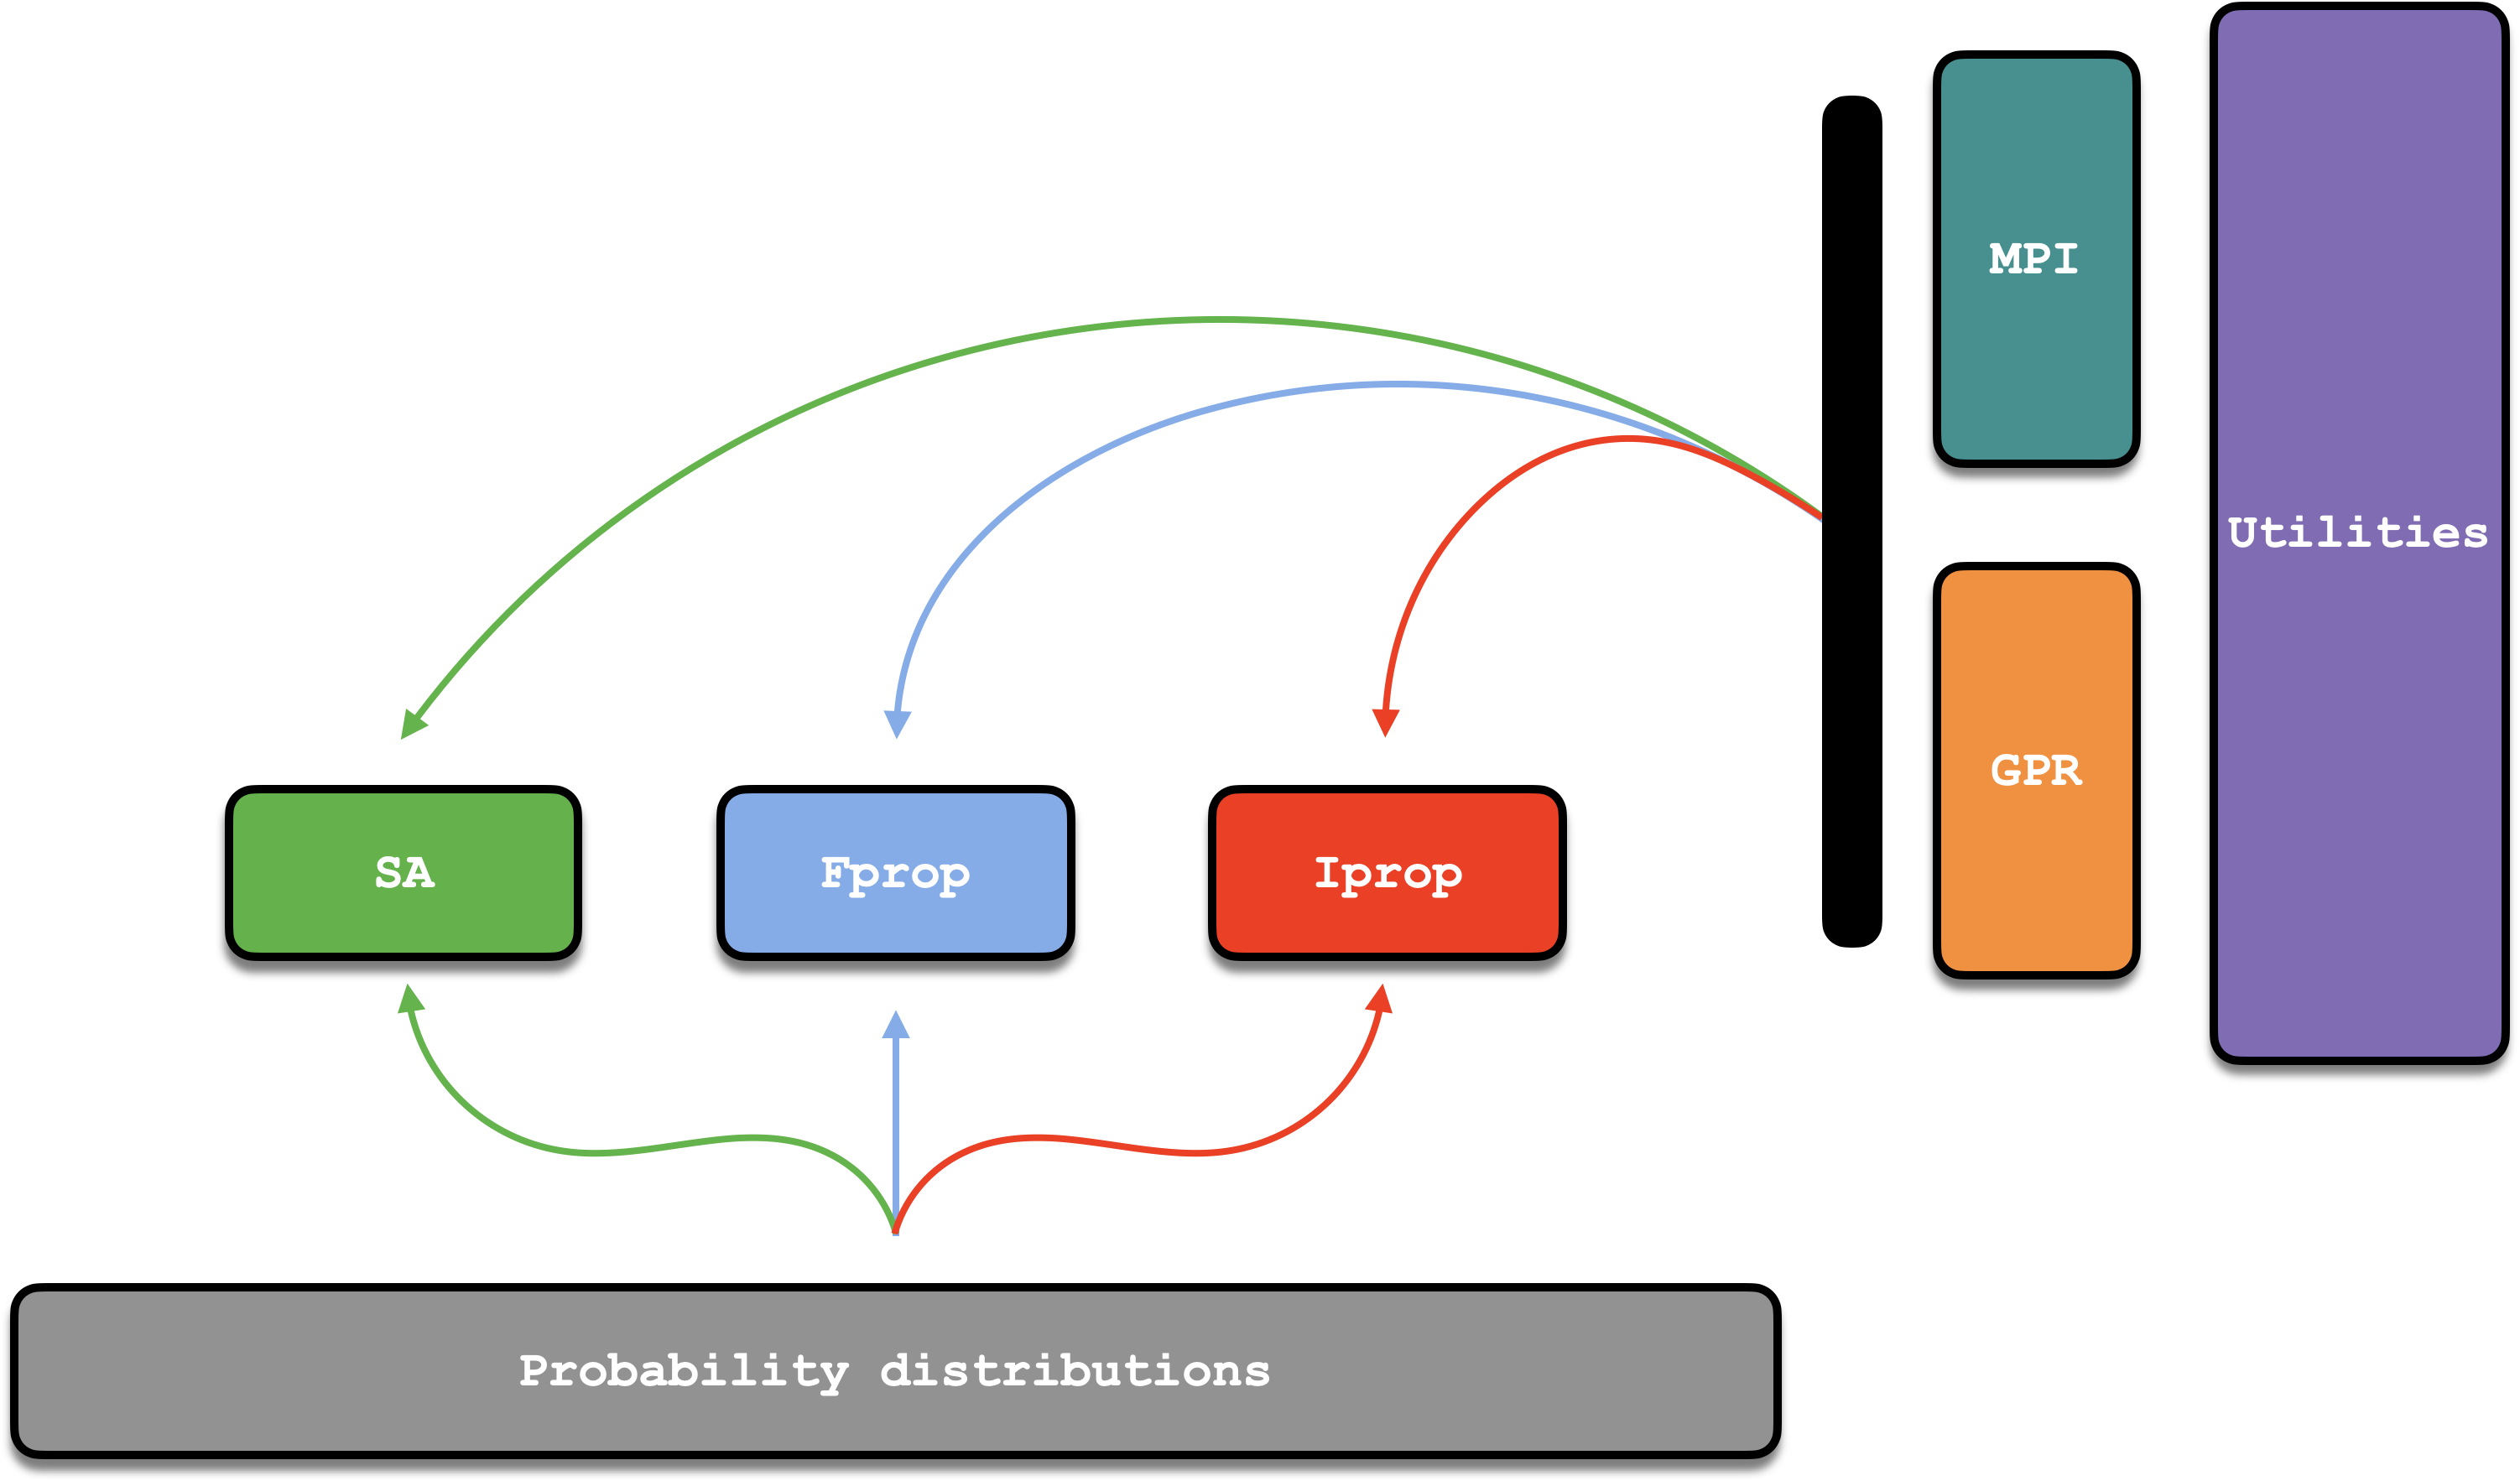
\includegraphics[width=0.9\textwidth]{./figures/block_diagram.png}
    \caption{The different blocks composing the SoFIA library.}
    \label{fig:blocks}
\end{figure}

Apart from the above-mentioned modules, a strong component of the SoFIA library is the applications within aerothermodynamics. In particular, two different modules are included: \texttt{catalysis} and \texttt{nitridation}. Fig.~\ref{fig:app_blocks} shows the different relationships among the different blocks. Seldom databases with the GPR models and data, such as parameter priors and measured quantities, are provided for each experimental case. Combining the different methods included in SoFIA, the user has an array of things that can be computed for material and flow characterization as well as diagnostics.

\begin{figure}[!htb]
    \center
    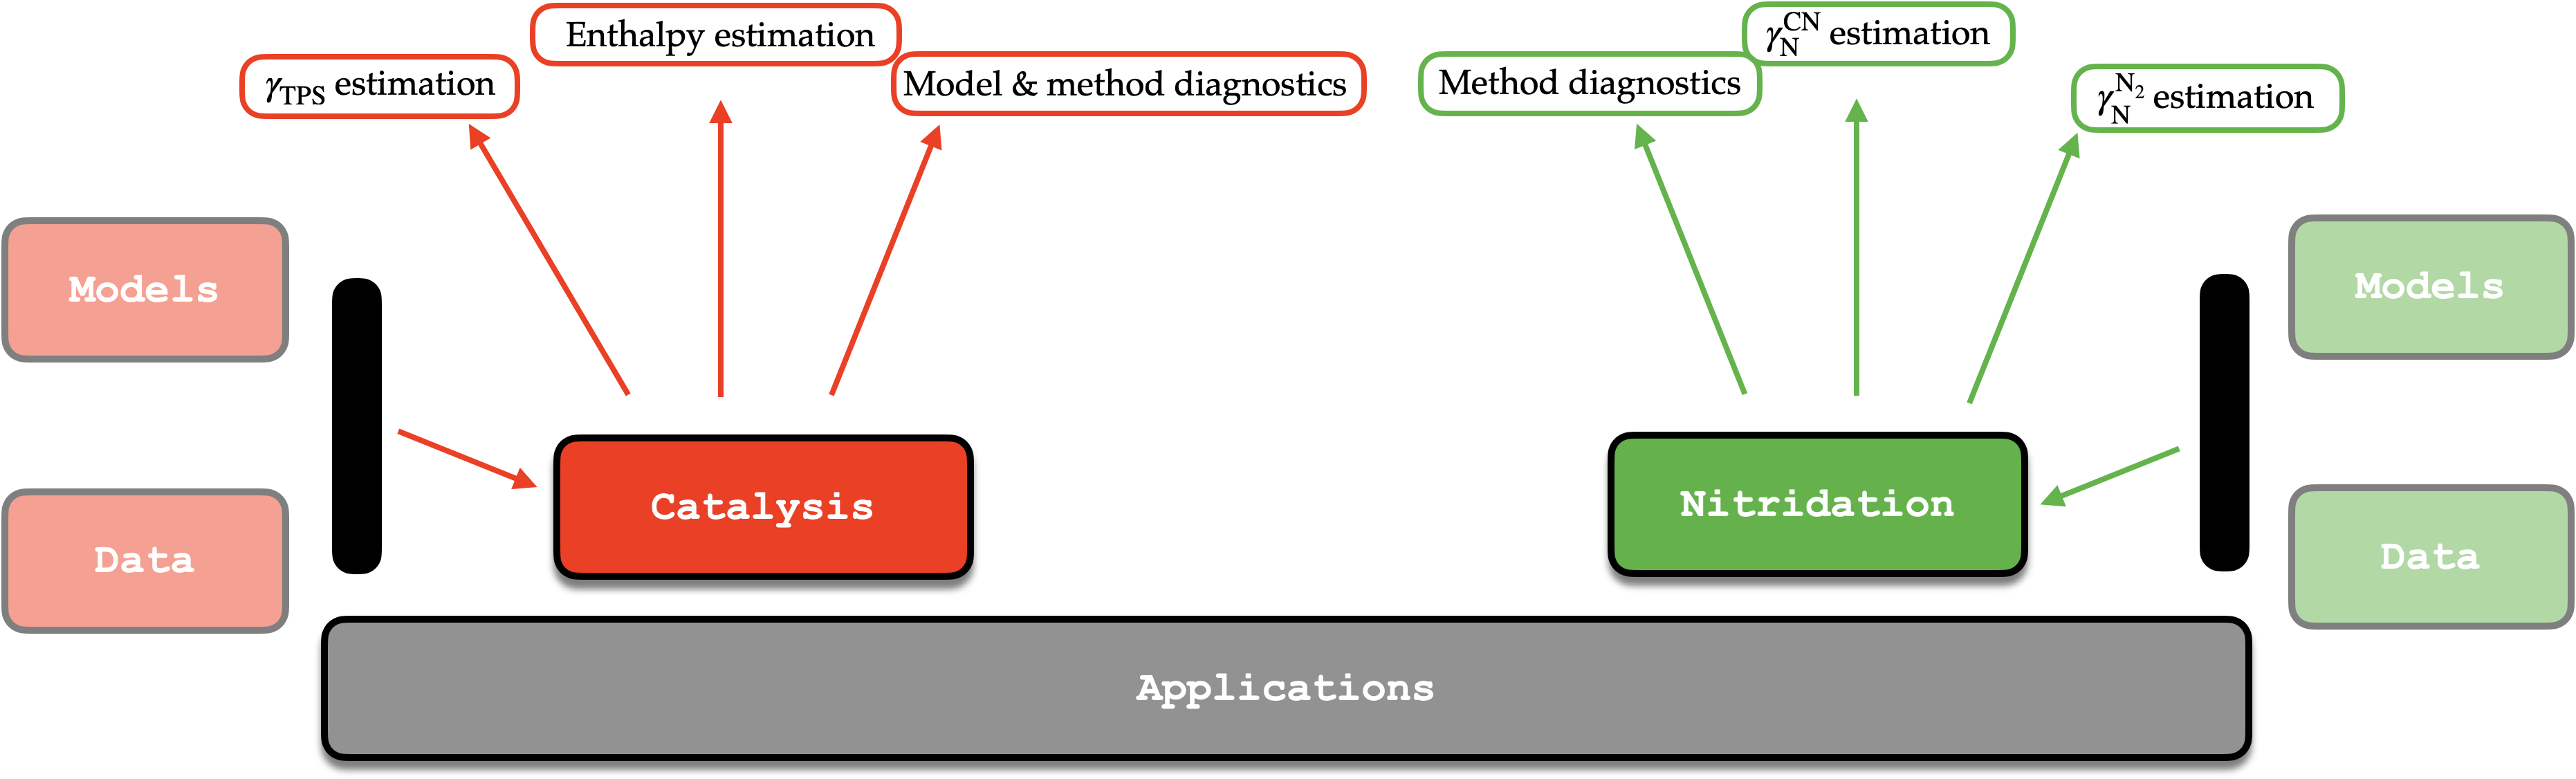
\includegraphics[width=\textwidth]{./figures/App_blocks.png}
    \caption{The different blocks composing the \texttt{Applications} module in the SoFIA library.}
    \label{fig:app_blocks}
\end{figure}

SoFIA not only offers an account of useful mathematical tools but also a principled and centralized way of storing models and data for the different applications.

\section{Usage}

In this section, we describe the basic imports and object calls to use the different features of the SoFIA library.\\

\noindent\textbf{\small Probability distributions (\texttt{Probability\_distributions}).} This module can be found in \texttt{SoFIA/Probability\_distributions}. Several utilities are defined in \texttt{distributions}\texttt{.py}. There are two implementations: uniform distribution and Gaussian distribution. Both objects can be used with an arbitrary number of dimensions, although the resulting n-dimensional distributions do not account for correlation among variables. To instantiate a distribution object we prescribe the number of dimensions and the hyperparameters: lower and upper bounds for uniform distributions, and mean and standard deviation for Gaussian distributions. We can then compute PDF values, log-PDF values (useful for inverse problems), CDF values, inverse CDF values (to sample arbitrary distributions based on uniform or Gaussians), and sample from the distribution itself. A code snippet with a usage example is shown hereafter.\\

\quoteON
```
\texttt{import sofia.distributions as dist}\\

\texttt{hyp = [[a,b]] \# Hyperparameters for a 1D distribution}\\

\texttt{D = dist.Uniform(n\_dimensions,hyp) or dist.Gaussian(n\_dimensions,hyp) \# Instantiation of probability distribution object: either 1D uniform or Gaussian}\\

\texttt{x = np.linspace(-10.,10.,1000)}\\

\texttt{D.get\_cdf\_values(x) \# get CDF values of the distribution}\\

\texttt{D.get\_samples(n\_samples) \# Sample the distribution}

```
\quoteOFF

\noindent\textbf{\small Sensitivity Analysis (\texttt{SA}).} This module can be found in \texttt{SoFIA/SA}. In there, you can find the \texttt{Sobol.py} file with different utilities. We have the \texttt{sampling\_sequence} which generates the matrices with the inputs that need evaluations from our model, and \texttt{indices} which takes on the resulting evaluations and compute the first and total order Sobol' indices. You can print out the matrix with the inputs (each row contains all the inputs for one evaluation of the model) and then generate the evaluations the way you prefer. Then you come back and get your indices. The following code snippet shows an example of usage of this module. In \texttt{[...]} you can include the body of your code, namely, the function you want to perform sensitivity analysis on and any other relevant characteristics.\\
\quoteON
```
\texttt{import sofia.Sobol as sbl}\\

\texttt{[...] \# Definition of the function to be evaluated}\\

\texttt{SA = sbl.Sobol() \# Instantiation of sensitivity analysis object}\\

\texttt{samples = SA.sampling\_sequence(n\_samples,n\_variables,['dist vars'],None)}\\

\texttt{[...] \# Evaluation of function f on the samples computed}\\

\texttt{SA.indices(f,n\_samples,n\_variables)}

```
\quoteOFF

The concrete example with the Ishigami function can be found in \texttt{SA/example.py}.\\

\noindent\textbf{\small Inverse uncertainty propagation (\texttt{Iprop}).} This module is placed in \texttt{SoFIA/Iprop}. Utilities can be found in the script \texttt{sampler.py} with which a Markov chain based on the Metropolis Hastings algorithm can be built. For the instantiation of the sampler we have to specify an initial covariance function \texttt{covinit}, a loglikelihood function \texttt{fun\_in}, and the number of samples to burn for the adaptation of the covariance matrix \texttt{nburn}. The chain is initiated with the parameters specified in the utility \texttt{seed}, while the \texttt{Burn} routine adapts the covariance matrix with the presribed number of draws \texttt{nburn}. The function \texttt{DoStep} advances the Markov chain and generates the useful samples to be used in the analysis of the posterior distribution. The script \texttt{sampler.py} also includes two diagnostic techniques: the plotting of the trace through the \texttt{chain\_visual} function, and the computation of the autocorrelation function with \texttt{autocorr}. For the chain diagnostics object, we must specify the chain samples and a dictionary that links the position of the variables in the vector of variables used for the chain construction to a variable name for plotting purposes. A code snippet with the typical usage of this module is shown hereafter.\\

\quoteON
```
\texttt{import sofia.sampler as mcmc}\\

\texttt{[...] \# Model to be calibrated and corresponding definition of the loglikelihood function of the experiments}

\texttt{sampler = mcmc.metropolis(np.identity(n\_dim)*0.01, log\_lik, n\_samples) \# Instantiation of the MCMC sampler}\\

\texttt{[...] \# Definition of the initial values of the parameters to be calibrated}\\

\texttt{sampler.seed(initial\_values\_of\_parameters)}\\

\texttt{sampler.Burn()}\\

\texttt{for i in range(n\_samples):}\\
\texttt{sampler.DoStep(1)}\\

\texttt{sampler\_diag = mcmc.diagnostics(chain,dict\_var) \# Instantiation of the chain diagnostics object}\\

\texttt{sampler\_diag.chain\_visual(n\_plots,var)}\\

\texttt{sampler\_diag.autocorr(n\_lags,n\_plots,var)}

```
\quoteOFF

\noindent\textbf{\small Forward uncertainty propagation (\texttt{Fprop}).} This module is placed in \texttt{SoFIA/Fprop}. For the moment, it includes a simple polynomial chaos construction. Sample-based methods can be built with the functionalities already included in the library. \\

\quoteON
```
\texttt{import sofia.pc as pce}\\
\texttt{import sofia.distributions as dist}\\

\texttt{\# Generate Gaussian samples to use}\\

\texttt{N = n\_samples}\\

\texttt{\# Definition of the distribution used in the PCE construction}\\

\texttt{hyp=[[0.,1.]]}\\
\texttt{G = dist.Gaussian(1,hyp)}\\
\texttt{S = G.get\_samples(N)}\\

\texttt{\# Definition of the targetted distribution}\\

\texttt{hypU=[[0.,1.]]}\\
\texttt{target = dist.Uniform(1,hypU)}\\

\texttt{h = target.fun\_icdf() \# Definition of the inverse CDF function of the target distribution}\\

\texttt{ki\_uniform = pce.approximate\_rv\_coeffs(n\_polynomials, h)}\\
\texttt{k = pce.generate\_rv(ki\_uniform, S) \# With k we should recover the target distribution}

```
\quoteOFF

\noindent\textbf{\small Applications (\texttt{Applications}).} This module can be accessed in \texttt{SoFIA/Applications} It includes scripts with which to reproduce the results obtained in my PhD thesis. These scripts put together different modules from SoFIA to perform all the computations. The only inputs to be provided are the external model evaluations and inputs from which to construct Gaussian process surrogates and carry out the inverse and/or forward analyses. The data from the simulations I used in my thesis are also available in different \texttt{json} files. The applications here included are related to the estimation of catalysis and nitridation parameters for TPS materials, as well as an adiabatic reactor example. For code snippets and examples of their usage, the reader is directed to \texttt{SoFIA/Docs/jup\_notebooks/env}. That folder contains a virtual environment with the jupyter notebooks \texttt{catalysis\_demo.ipynb, nitridation\_demo.ipynb}, and \texttt{Adiabatic\_reactor.ipynb}. Some particular examples are offered in the next section.\\

\section{Examples}

Particular examples of the usage of the different modules depicted in the previous section can be found in \texttt{SoFIA/examples}. Here we describe some of them and show the results for verification purposes.\\

\noindent \textbf{\small Probability distributions (\texttt{Probability\_distributions}).} In the example \texttt{Probability} \texttt{\_distributions}\texttt{/examples/example.py} we compute 1D and 2D uncorrelated uniform and Gaussian distributions. We first sample a uniform distribution with support $\mathcal{U}[-8,8]$ for which we generate 1000 samples and compute the CDF and PDF.

\begin{figure}[!htb]
    \centerline{
    \begin{tabular}{c c}
    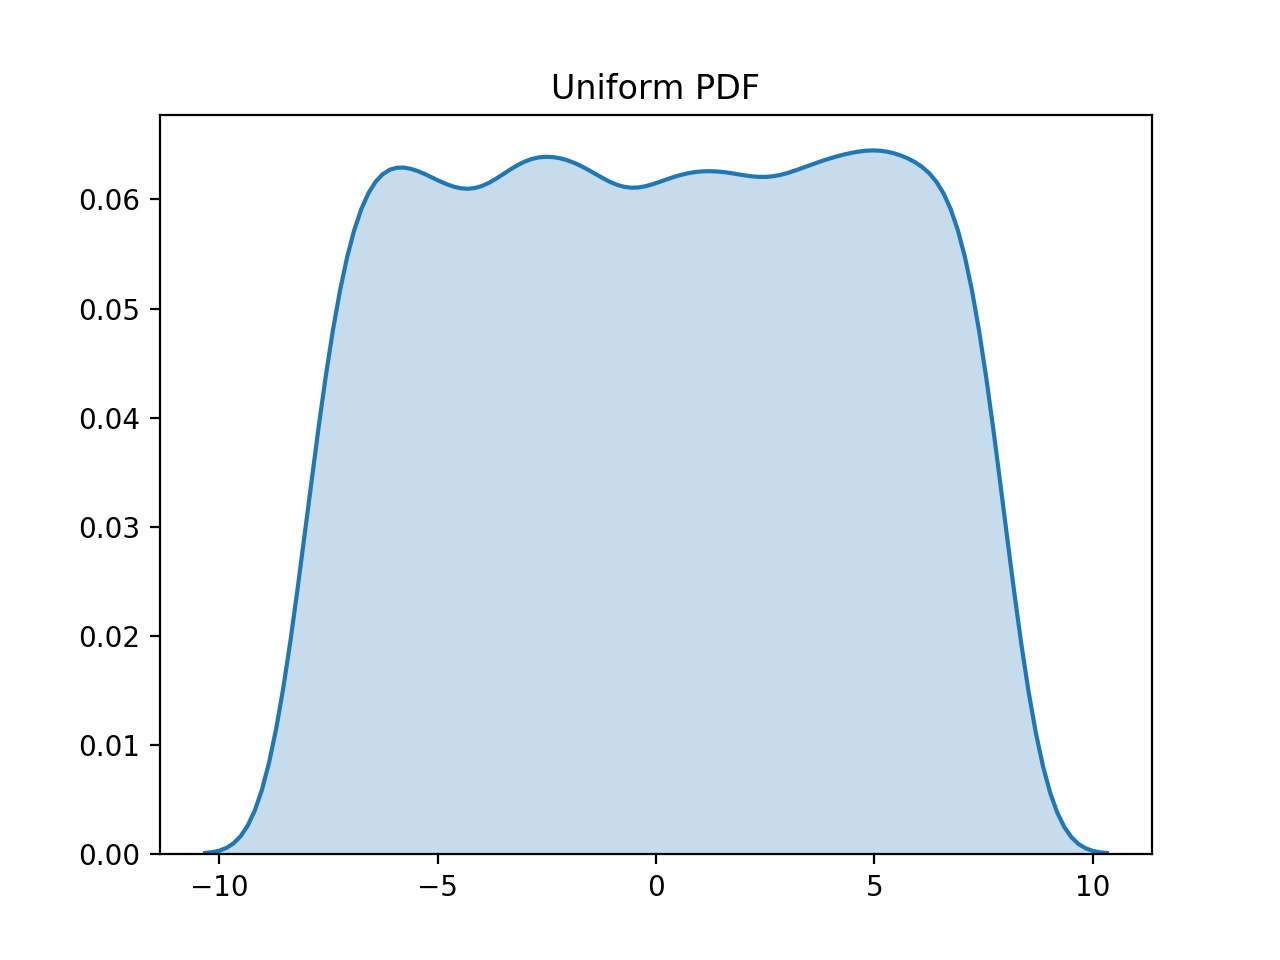
\includegraphics[width=0.5\textwidth]{./figures/uniform_pdf.png} &
    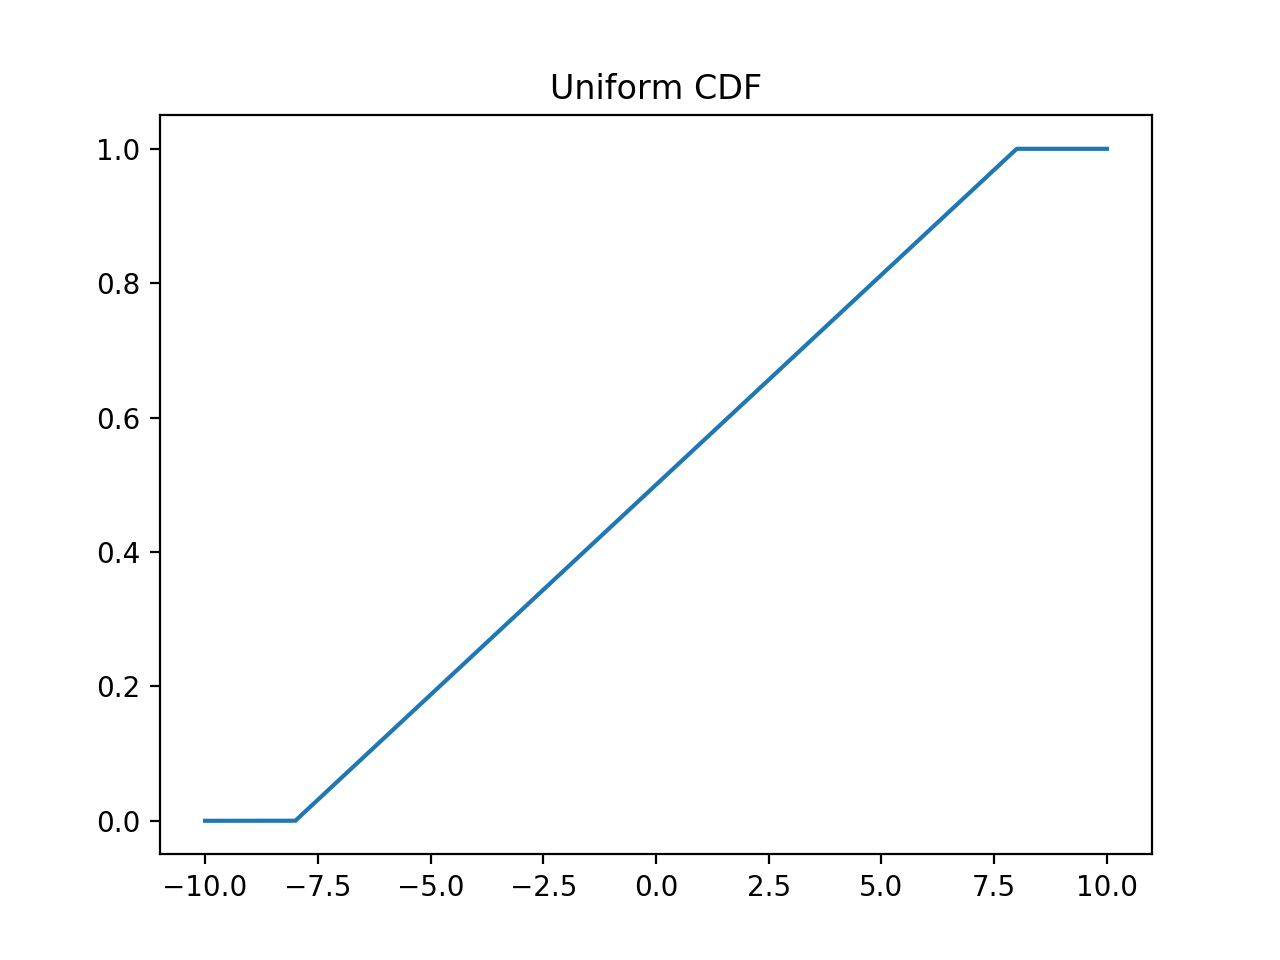
\includegraphics[width=0.5\textwidth]{./figures/uniform_cdf.png} 
    \end{tabular}}
    \caption{1D uniform PDF and CDF.}
    \label{fig:1d_uniform}
\end{figure}

We do the same for a 1D Gaussian distribution $\mathcal{N}(\mu=-1, \sigma=4)$

\begin{figure}[!htb]
    \centerline{
    \begin{tabular}{c c}
    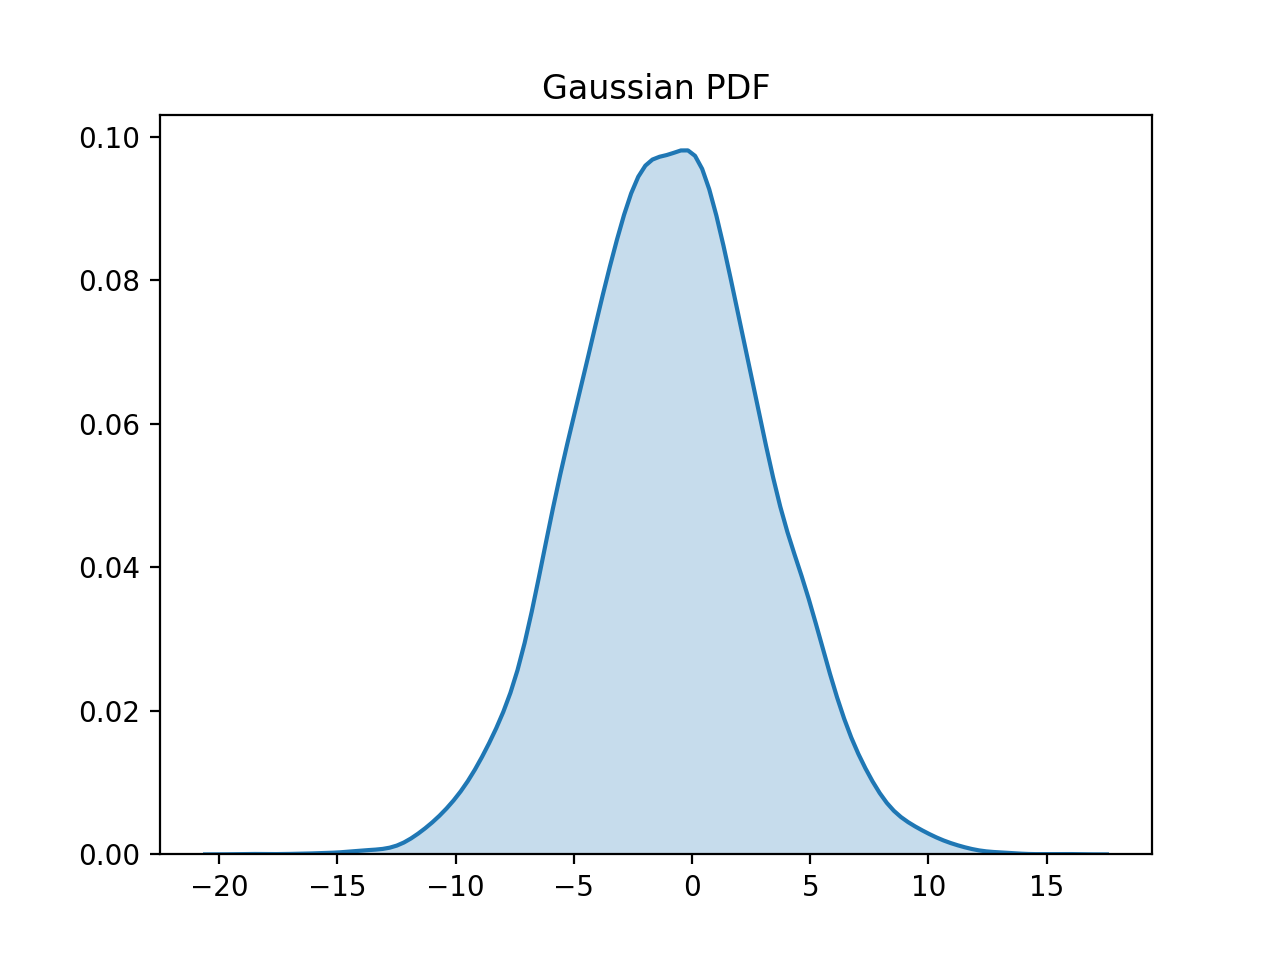
\includegraphics[width=0.5\textwidth]{./figures/gaussian_pdf.png} &
    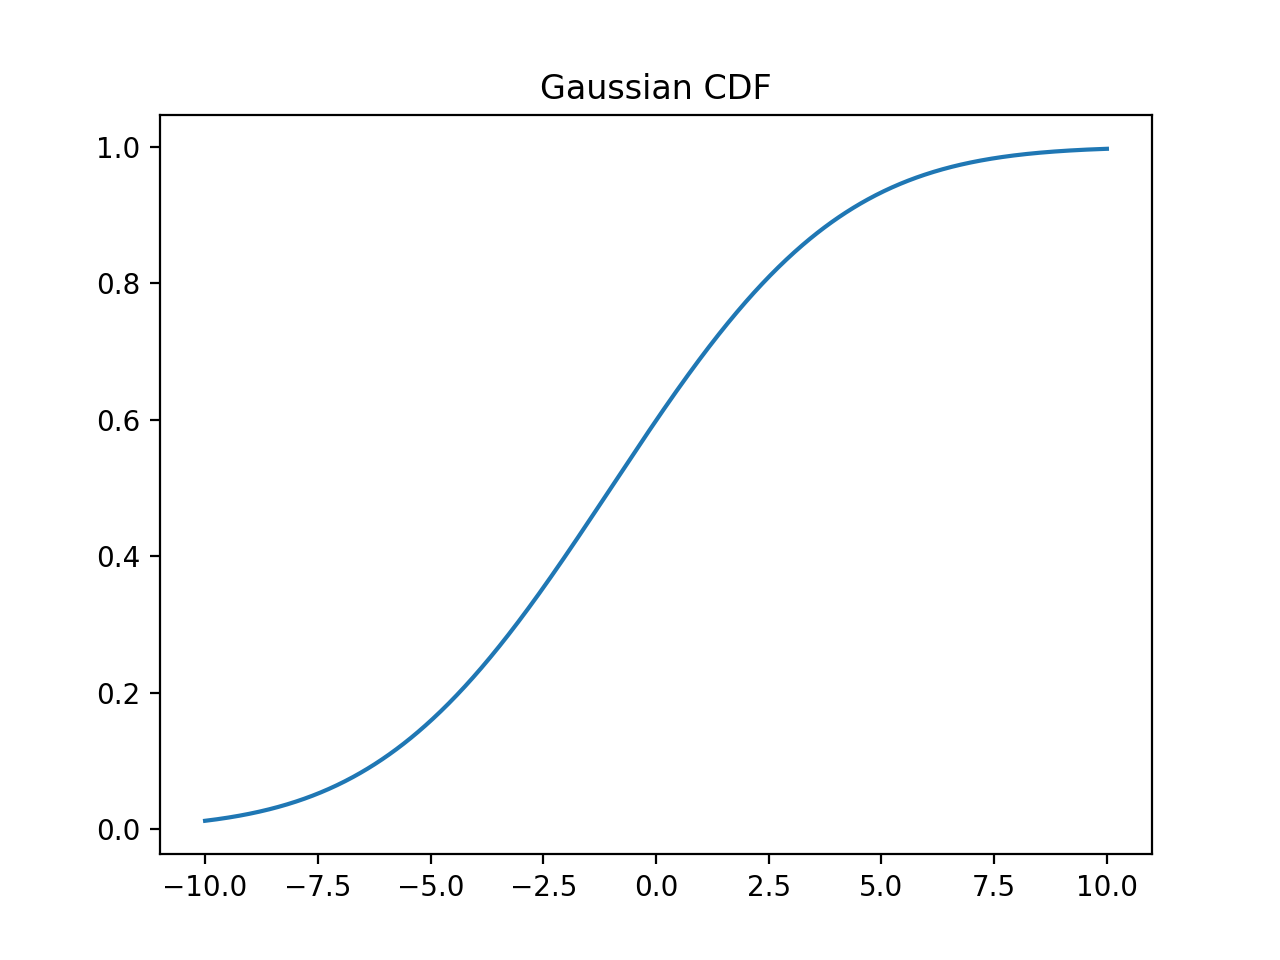
\includegraphics[width=0.5\textwidth]{./figures/gaussian_cdf.png} 
    \end{tabular}}
    \caption{1D Gaussian PDF and CDF.}
    \label{fig:1d_gaussian}
\end{figure}

We can also compute marginal CDFs and PDFs for 2D distribution of uncorrelated variables. In this case, the uniform distribution has for hyperparameters $\mathcal{U}[-1,4] \times \mathcal{U}[0,2]$, while the 2D Gaussian is defined $\mathcal{N}(-1,4) \times \mathcal{N}(0,2)$.\\

\begin{figure}[!htb]
    \centerline{
    \begin{tabular}{c c}
    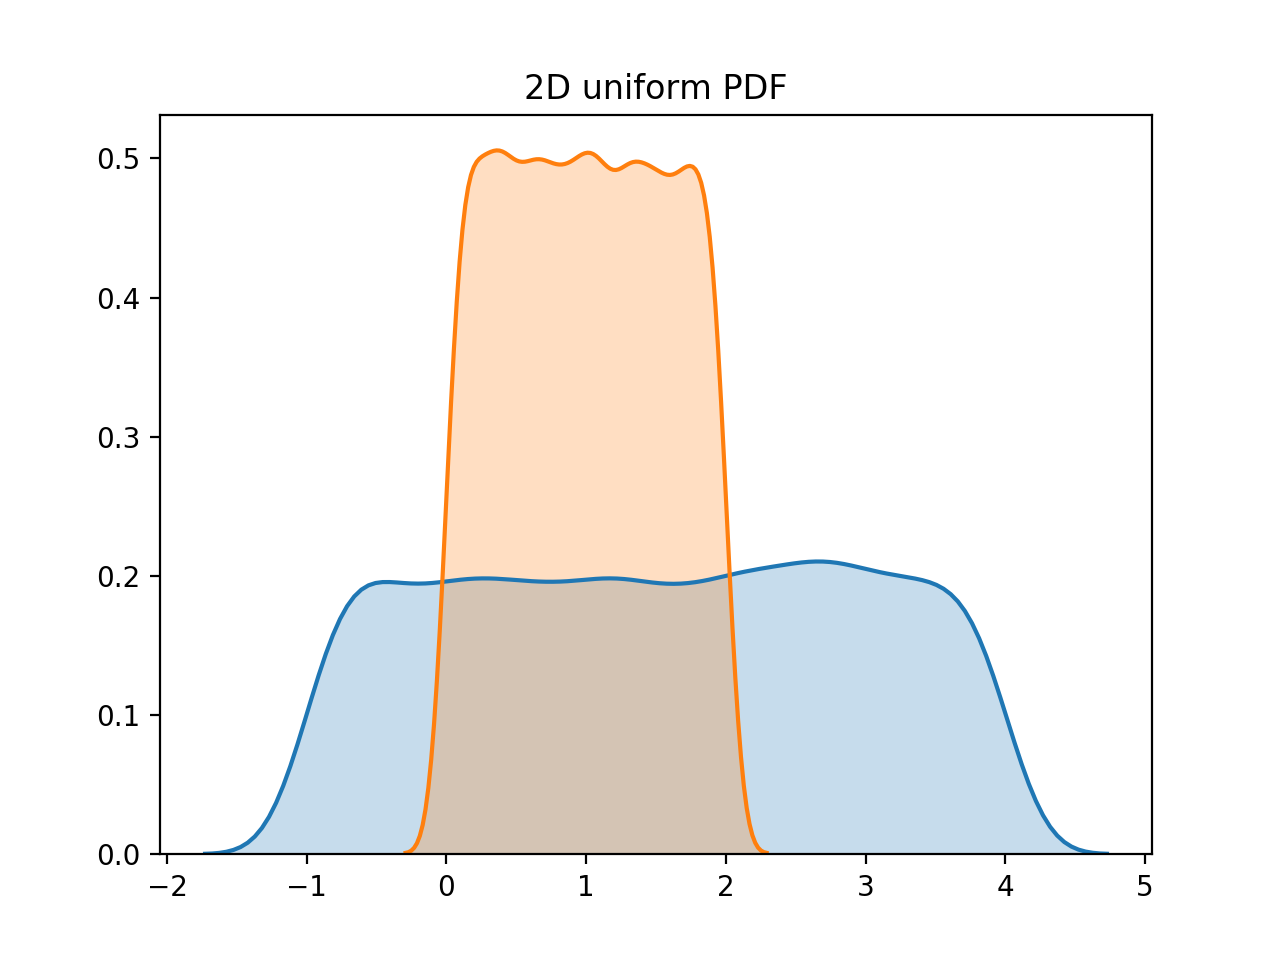
\includegraphics[width=0.5\textwidth]{./figures/marginal_uniform_pdf.png} &
    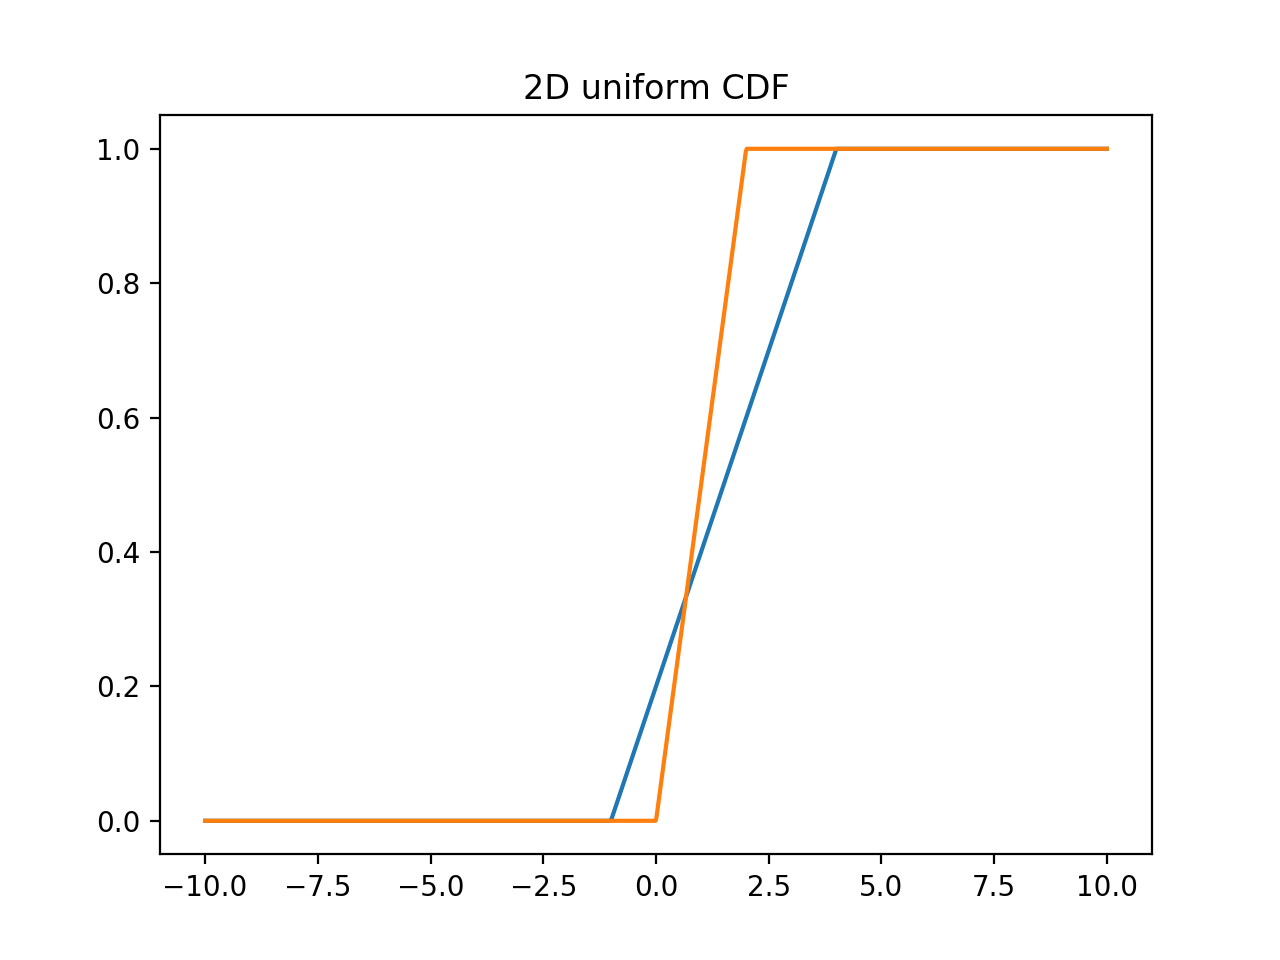
\includegraphics[width=0.5\textwidth]{./figures/marginal_uniform_cdf.png} \cr
    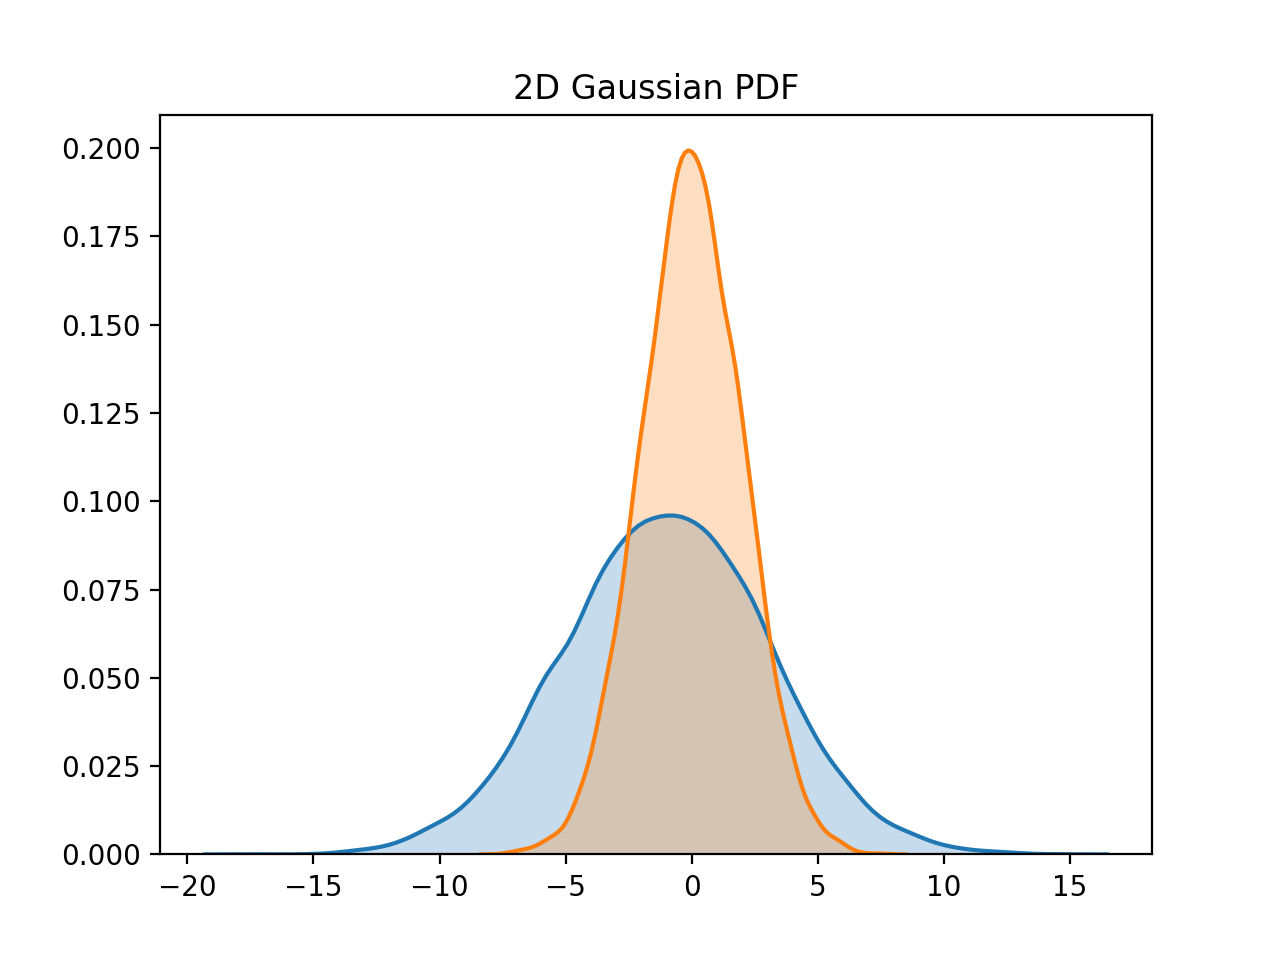
\includegraphics[width=0.5\textwidth]{./figures/marginal_gaussian_pdf.png} &
    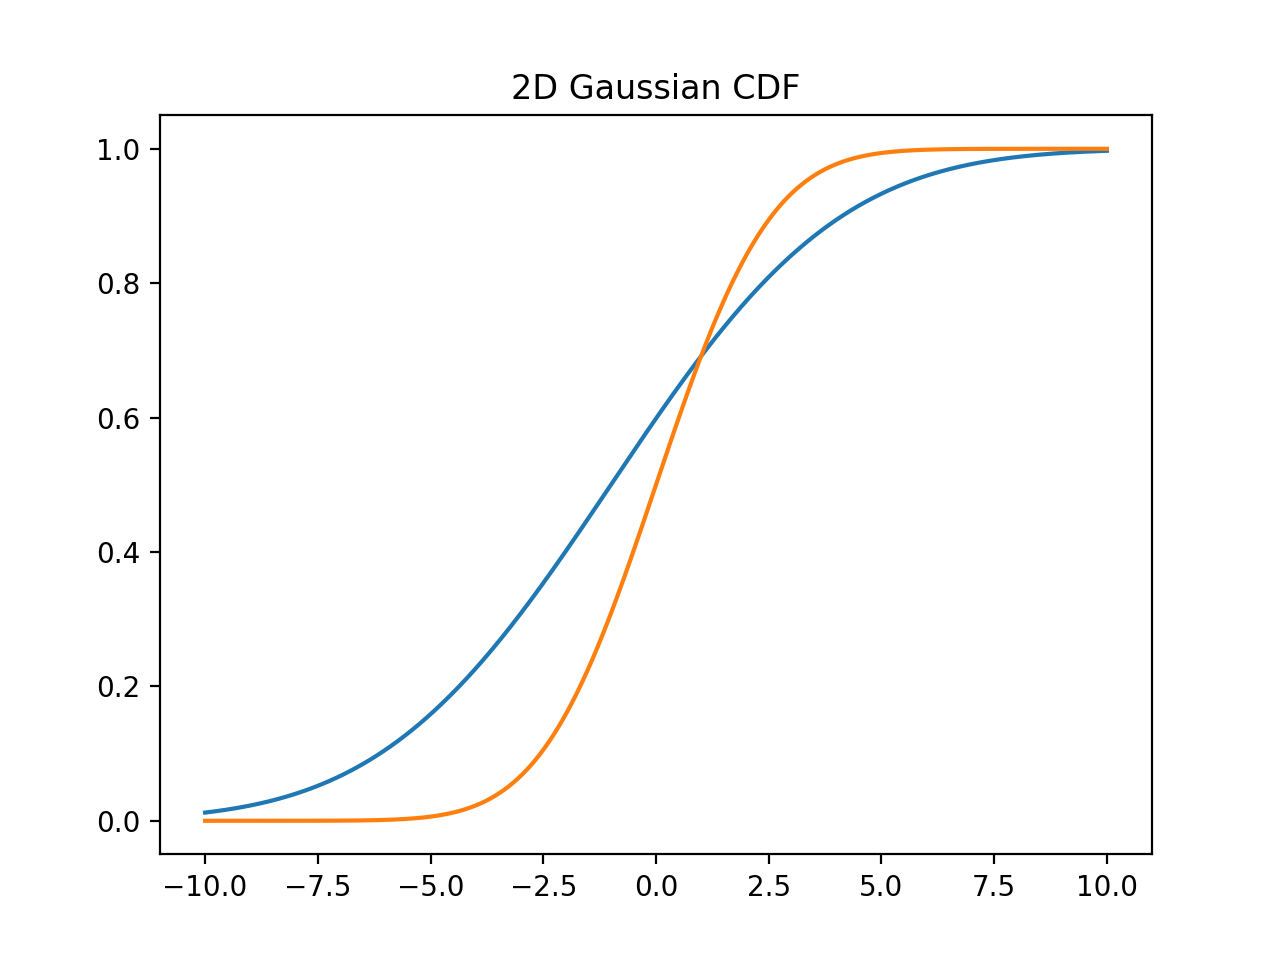
\includegraphics[width=0.5\textwidth]{./figures/marginal_gaussian_cdf.png}
    \end{tabular}}
    \caption{2D uniform and Gaussian marginal PDFs and CDFs.}
    \label{fig:1d_gaussian}
\end{figure}

\noindent \textbf{\small Sensitivity Analysis (\texttt{SA}).} In the example \texttt{SA/examples/example.py}, we work with the Ishigami function\\

\begin{equation}\label{eq:ishigami}
    f(x,y) = \sin(x) + a \cdot \sin(y)^{2} + b \cdot z^{4}\sin(x),
\end{equation}
for which we compute sensitivity indices for $x, y, z$ with respect to the model output $f$. The model parameters $a$ and $b$ are set to the values 7 and 0.1, respectively. We assume uniform distributions $\mathcal{U}[-\pi,\pi]$ for $x, y, z$ and base our estimations on 10,000 samples.

\begin{table}[!hbt]
    \centering
    \caption{Sobol' sensitivity indices for the inputs $x, y, z$ of the Ishigami function~\eqref{eq:ishigami}.} 
    \label{tab:models}
      \begin{tabular}{c  c  c}
        \toprule
        Variables  & $S_{i}$  & $S_{\mathrm{T}_{i}}$ \\ \midrule
        $x$ & 0.312 & 0.576\\
        $y$ & 0.446 & 0.443\\
        $z$ & 0.009 & 0.246\\
    
      \end{tabular}
\end{table}

\noindent \textbf{\small Inverse uncertainty propagation (\texttt{Iprop}).} There are several examples for this module. \\

\noindent\textbf{\small Example 1.} The first example \texttt{Iprop/examples/example\_ishigami.py} consists of inferring parameters $a$ and $b$ from noisy observations $f$ of the Ishigami function~\eqref{eq:ishigami}. In this case, the parameters are set to the values $a=8$ and $b=1$ while the noise of the observations is set to $\sigma=0.2$. The results are based on data in 3 different points $(x,y,z)$: $(0,1,2), (0,2,5)$, and $(1,8,5)$. The following figure~\ref{fig:ishigami_inverse} shows the trace for parameter $b$ and the marginal posteriors obtained for a 100,000 steps chain with an initial burn-in stage of 100,000 samples. The overall acceptance rate is 0.34008.

\begin{figure}[!htb]
    \centerline{
    \begin{tabular}{c c}
    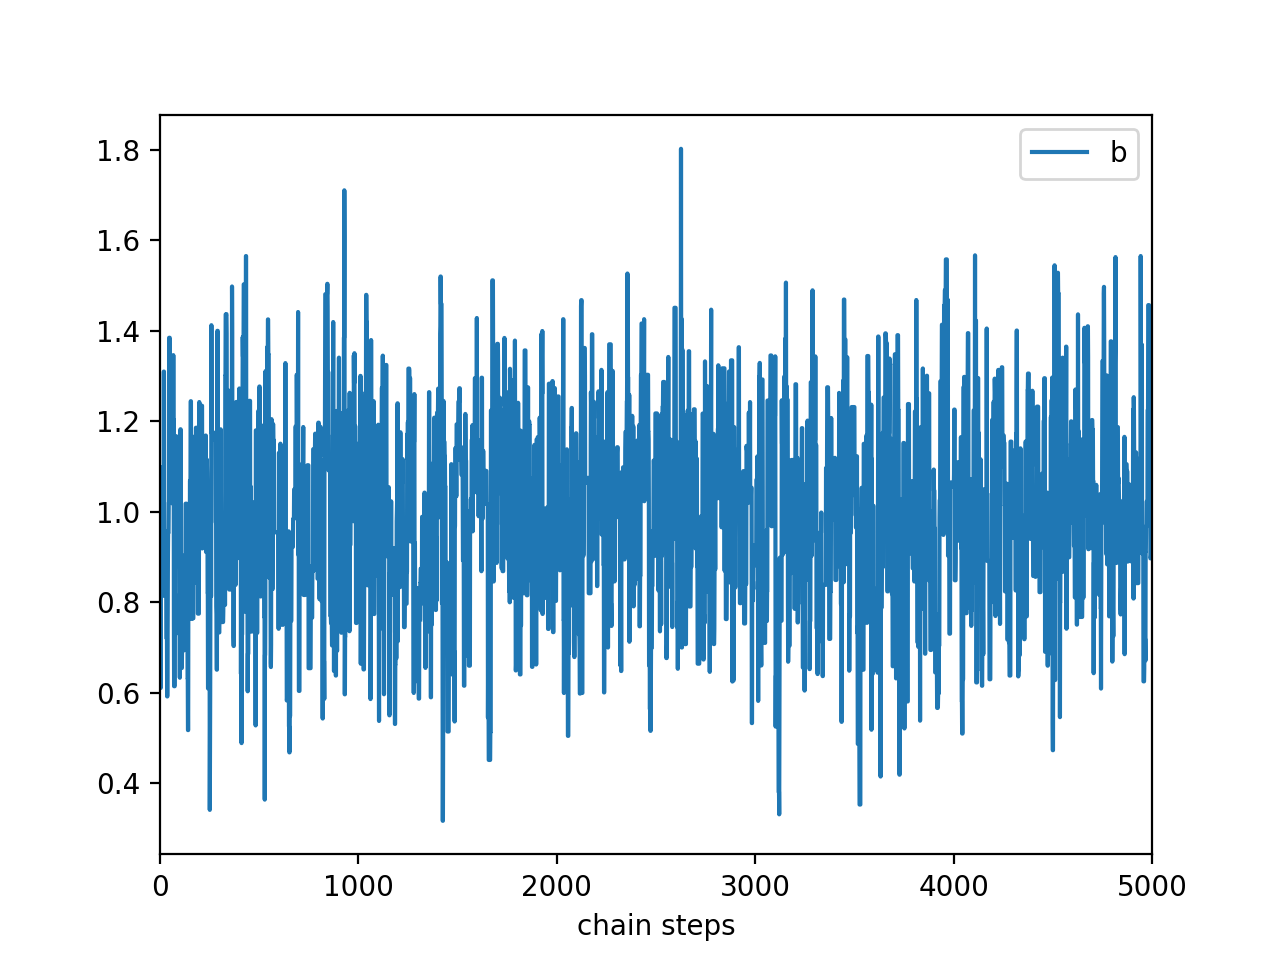
\includegraphics[width=0.5\textwidth]{./figures/ishigami_chain_trace.png} &
    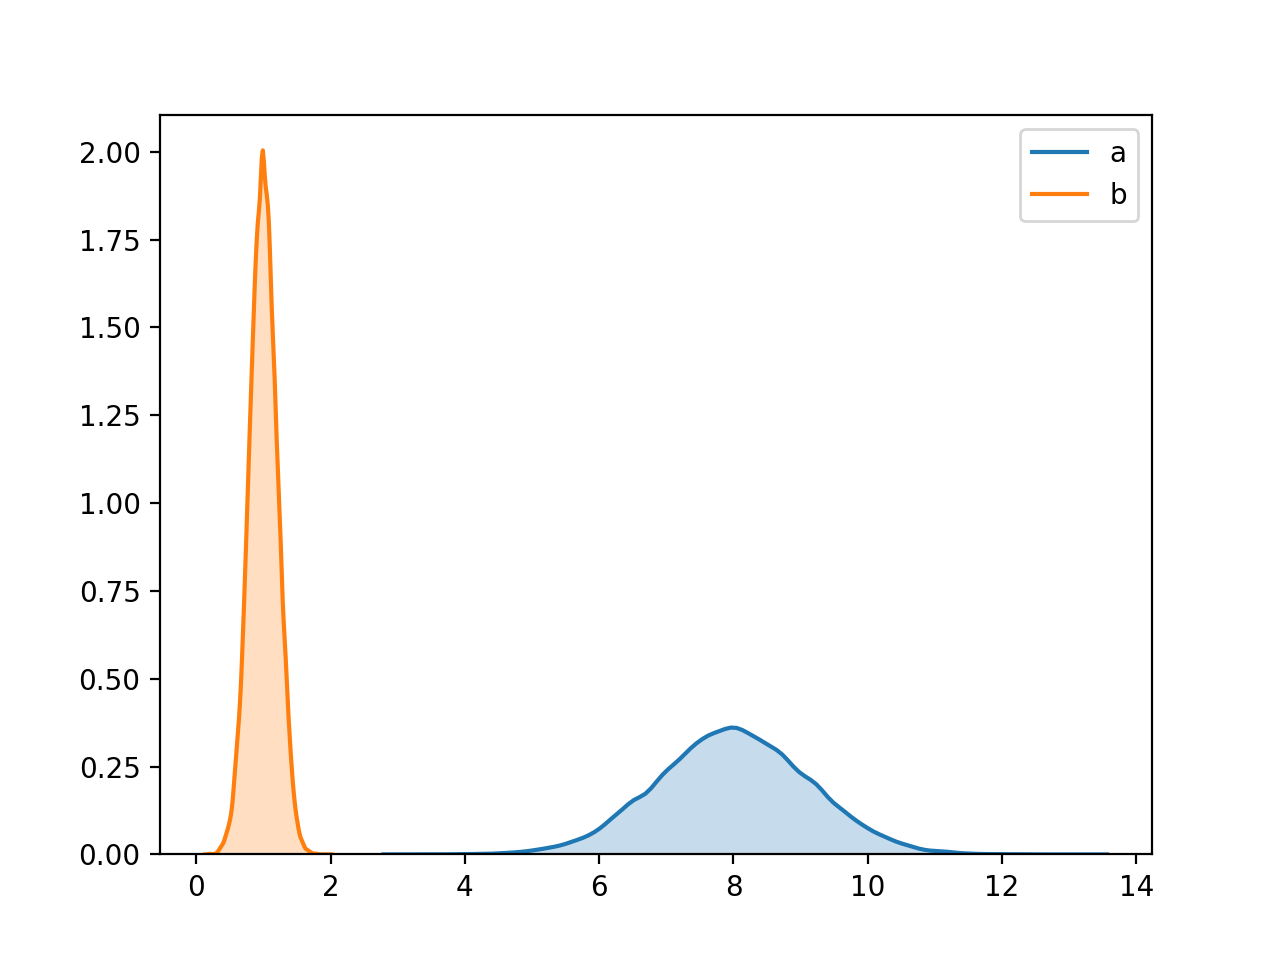
\includegraphics[width=0.5\textwidth]{./figures/ishigami_marginal_post.png}
    \end{tabular}}
    \caption{Left: chain trace for parameter $b$ for 5,000 steps. Right: marginal posterior distributions of parameters $a$ and $b$.}
    \label{fig:ishigami_inverse}
\end{figure}

We also show the autocorrelation function in the following figure

\begin{figure}[!htb]
    \centerline{
    \begin{tabular}{c c}
    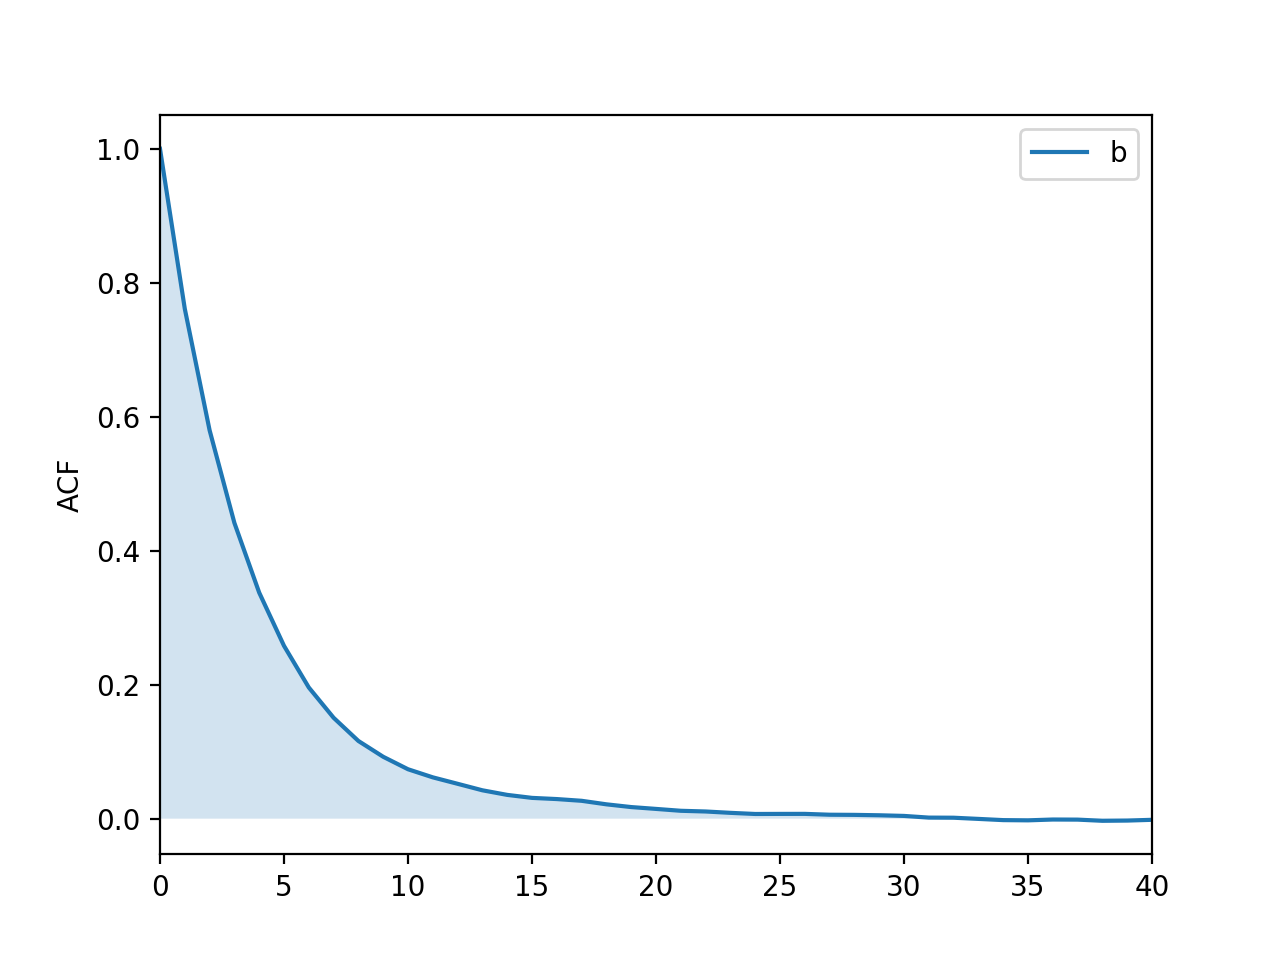
\includegraphics[width=0.5\textwidth]{./figures/ishigami_acf.png}
    \end{tabular}}
    \caption{Autocorrelation function of the chain for parameter $b$.}
    \label{fig:ishigami_acf}
\end{figure}

\noindent\textbf{\small Example 2.} Another example consists on the sampling of two Gaussian distributions by means of MCMC. We sample the Gaussians $\mathcal{N}(0,1)$ and $\mathcal{N}(5,1)$ whose true analytical PDFs are compared to the MCMC result through which the mean parameters $\mu_{1}$ and $\mu_{2}$ of the distributions are estimated. Figs~\ref{fig:mcmc_gaussian_pdf}-\ref{fig:mcmc_gaussian_chain_acf} show the results.

\begin{figure}[!htb]
    \centerline{
    \begin{tabular}{c c}
    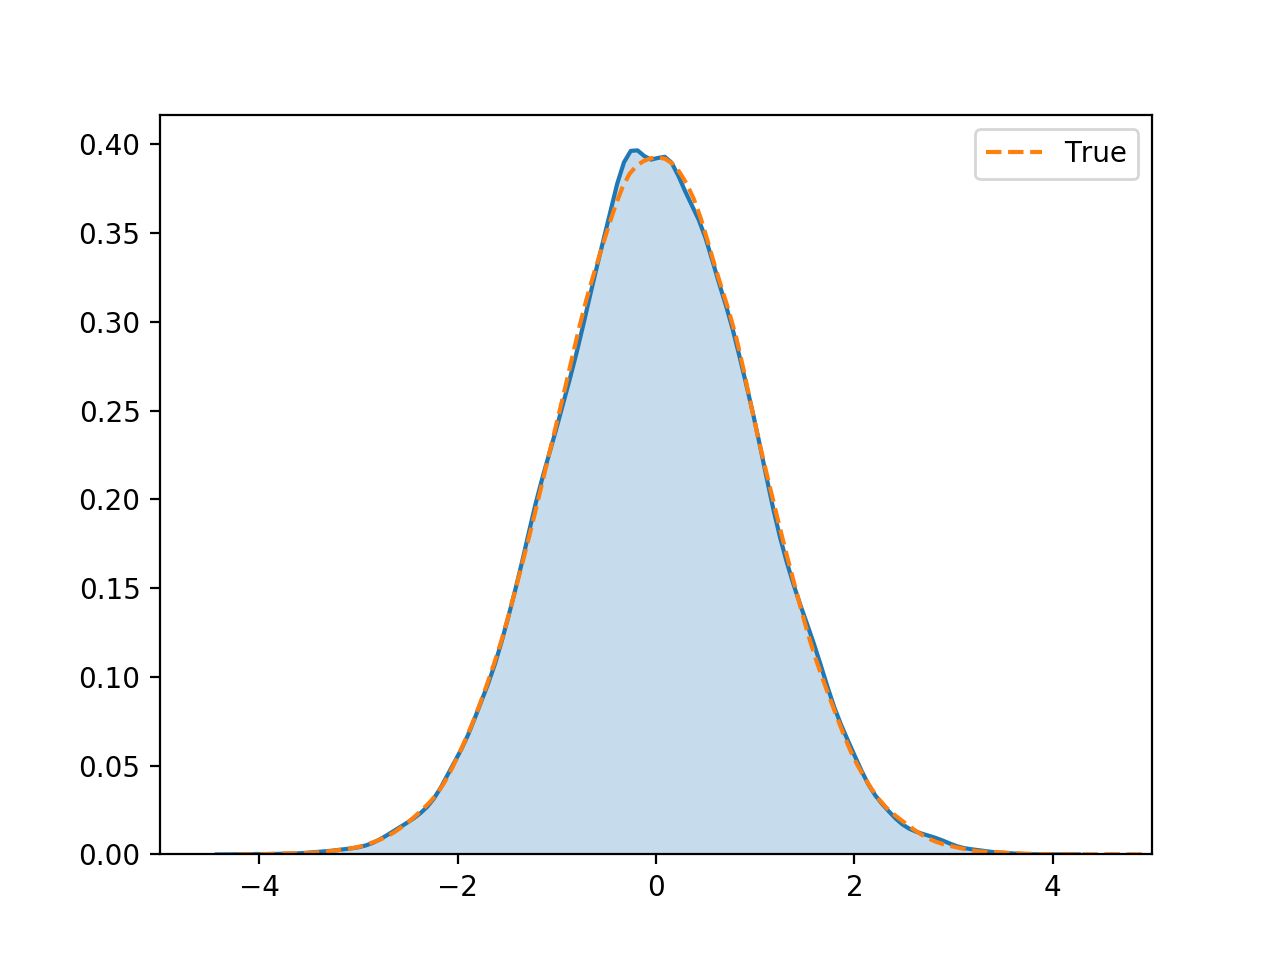
\includegraphics[width=0.5\textwidth]{./figures/mcmc_N01.png} &
    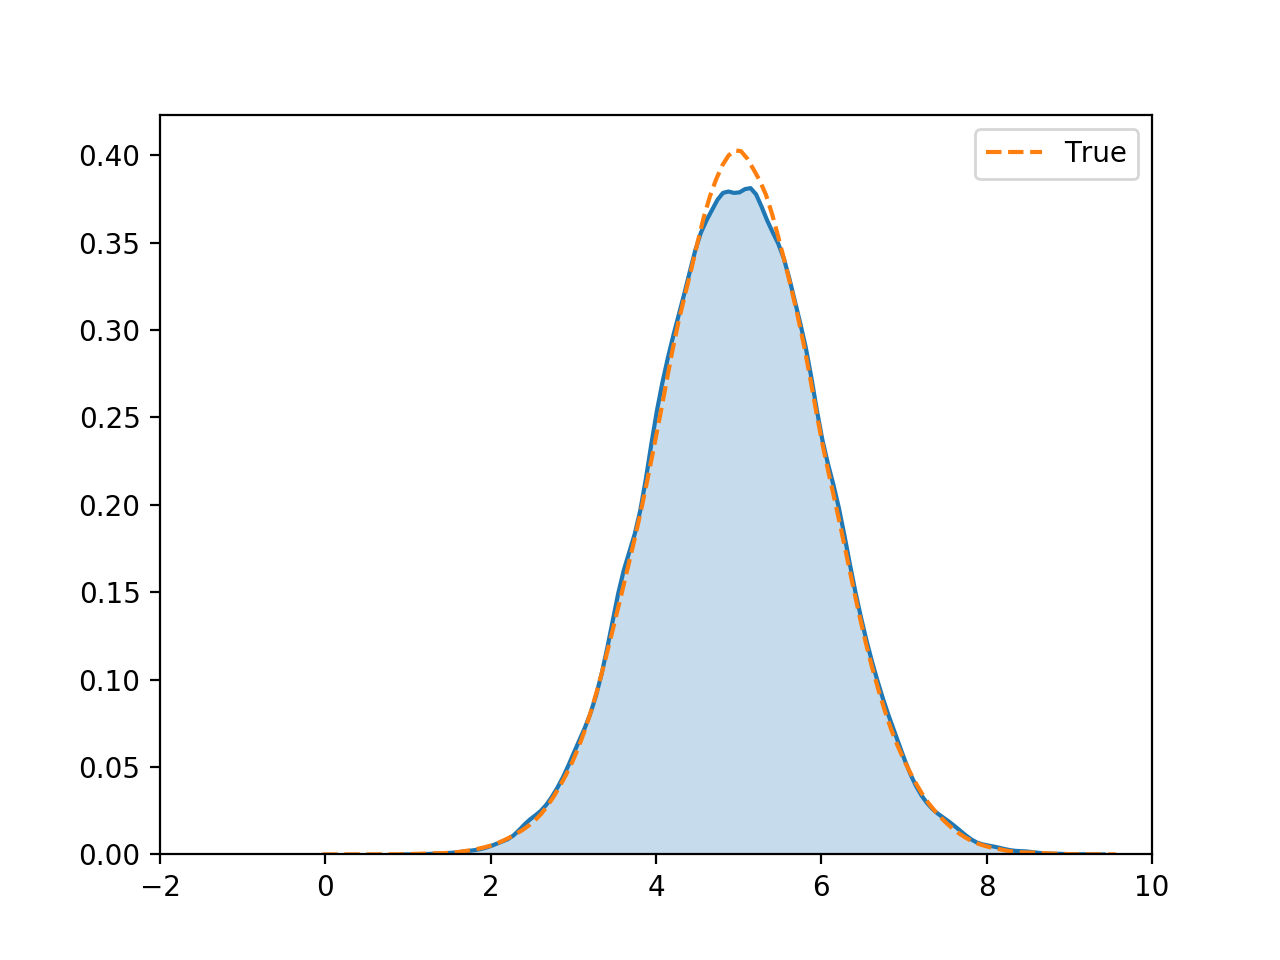
\includegraphics[width=0.5\textwidth]{./figures/mcmc_N51.png}
    \end{tabular}}
    \caption{Left: true PDF versus the PDF recovered from the Markov chain samples for the first Gaussian distribution $\mathcal{N}(0,1)$ Right: true PDF versus the PDF recovered from the Markov chain samples for the first Gaussian distribution $\mathcal{N}(5,1)$.}
    \label{fig:mcmc_gaussian_pdf}
\end{figure}

\begin{figure}[!htb]
    \centerline{
    \begin{tabular}{c c}
    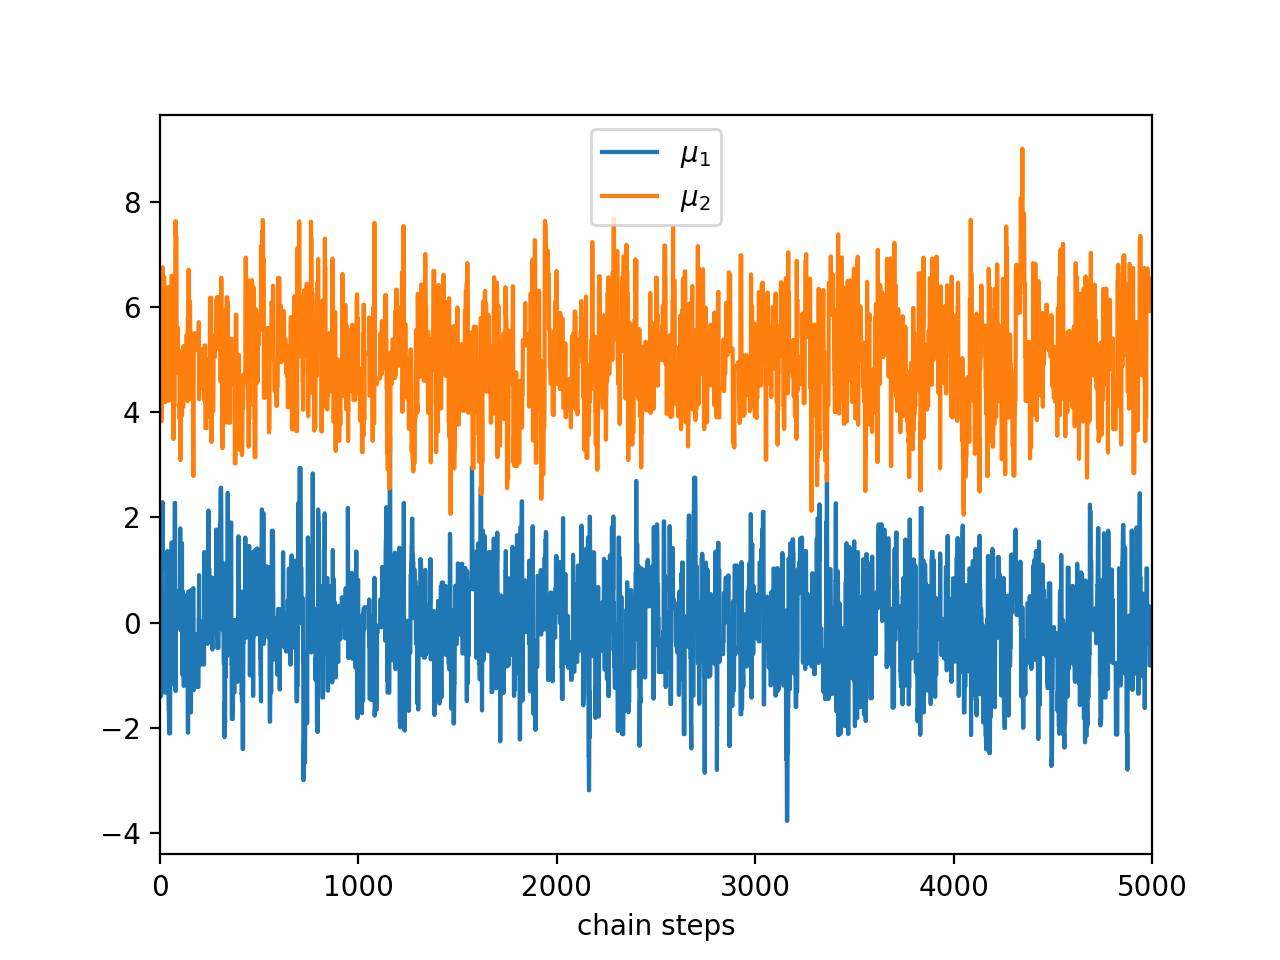
\includegraphics[width=0.5\textwidth]{./figures/mcmc_gaussian_chains.png} &
    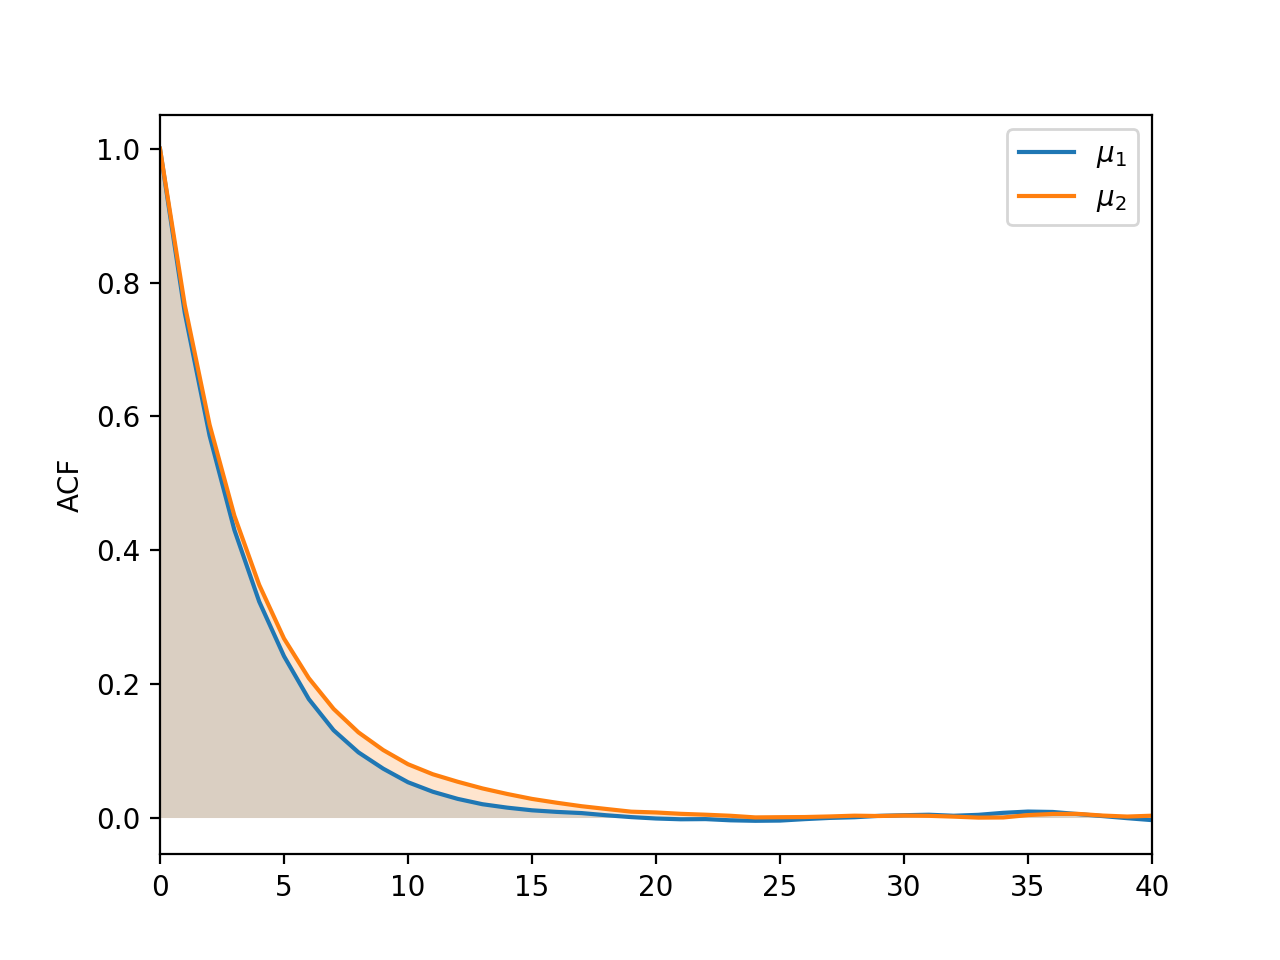
\includegraphics[width=0.5\textwidth]{./figures/mcmc_gaussian_acfs.png}
    \end{tabular}}
    \caption{Left: chain traces for parameters $\mu_{1}$ and $\mu_{2}$ of the Gaussian distributions we are sampling with a MCMC method for 5,000 steps. Right: autocorrelation functions.}
    \label{fig:mcmc_gaussian_chain_acf}
\end{figure}

\noindent\textbf{\small Example 3.} The last example included in the library consists of the reconstruction of a polynomial of arbitrary degree $k$, $f(x) = \sum_{k=0}^{q} a_{q}x^{q}$ from 30 noisy observations randomly sampled in the canonical range $x \in [0,1]$ with $\sigma=0.1$. We first fit the linear polynomial 

\begin{equation}
    f(x) = 10 -2 \cdot x
\end{equation}
by fixing $a_{0} = 10$, $a_{1} = -2$ and $a_{i} = 0, \ \ \forall i \in {2,...,4}$. The results of the posterior predictive check as well as the marginal posteriors of the parameters are shown in Fig.~\ref{fig:poly_lin}.

\begin{figure}[!htb]
    \centerline{
    \begin{tabular}{c c}
    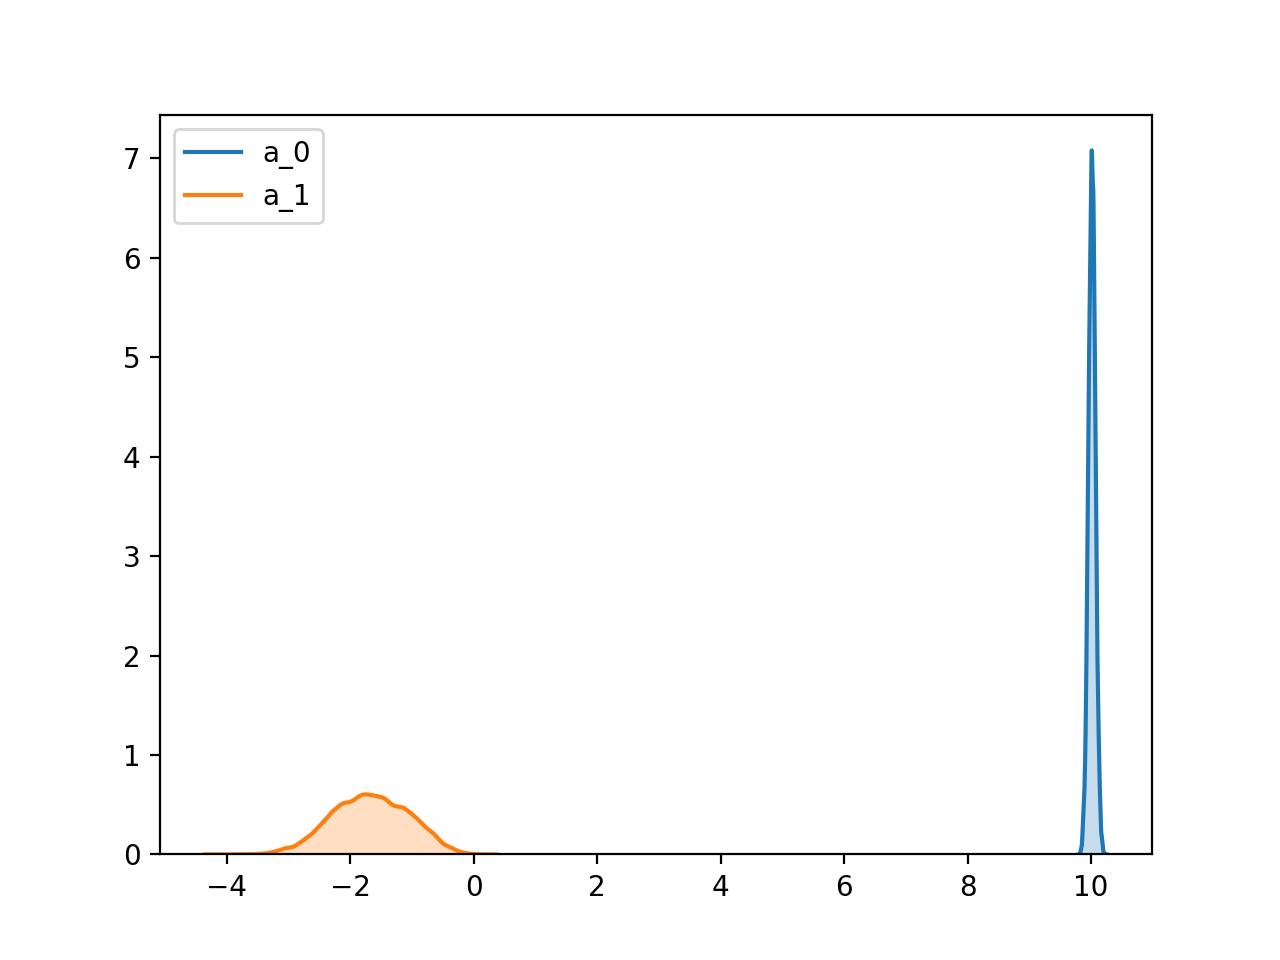
\includegraphics[width=0.5\textwidth]{./figures/linear_coeffs.png} &
    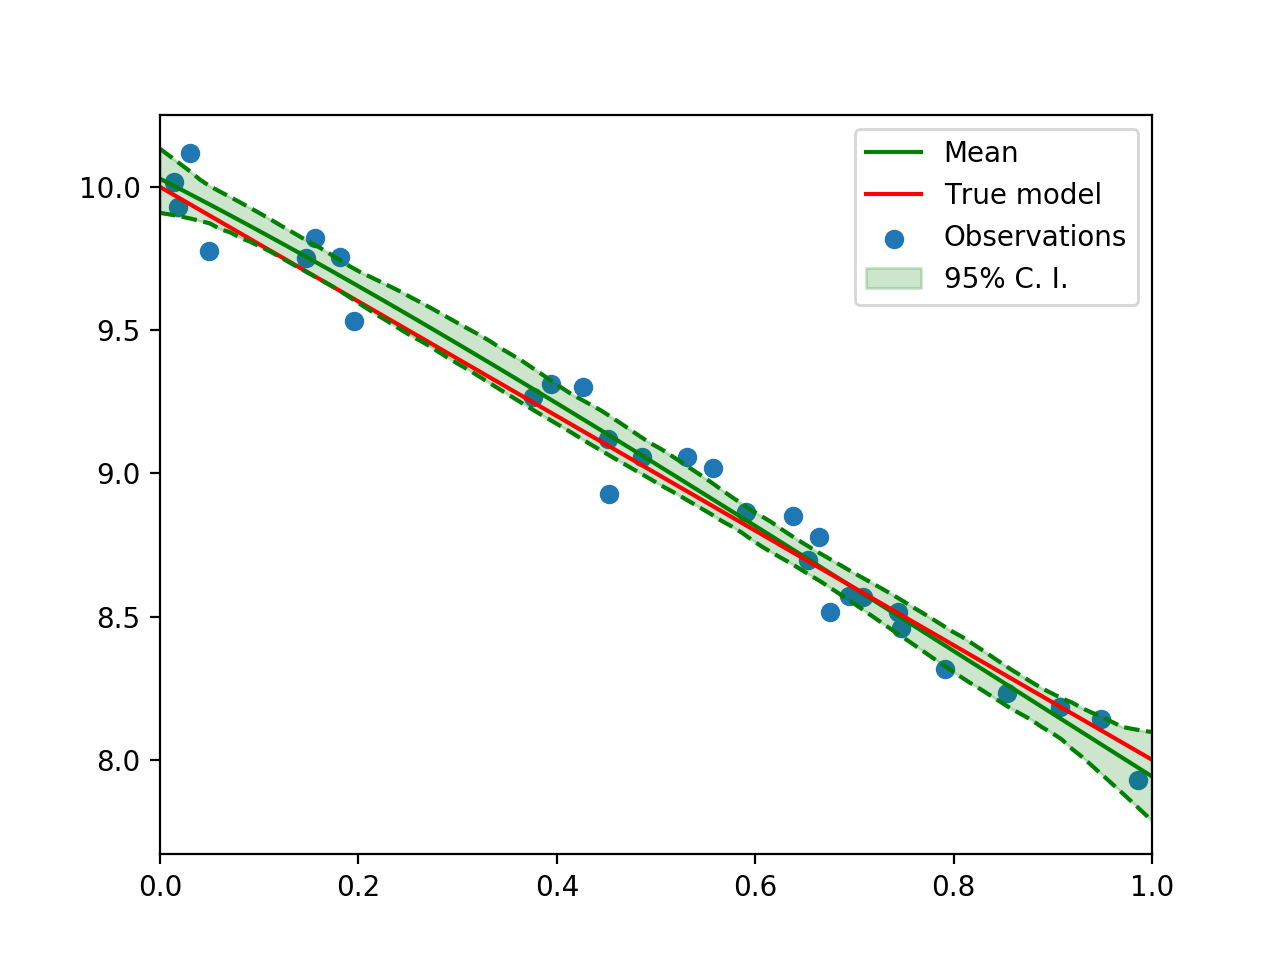
\includegraphics[width=0.5\textwidth]{./figures/linear_polynomial.png}
    \end{tabular}}
    \caption{Left: marginal posterior distributions for parameters $a_{0}$ (bias) and $a_{1}$ (slope) for the linear polynomial model. Right: posterior predictive check.}
    \label{fig:poly_lin}
\end{figure}

We then fit a more challenging model, $f(x) = 10 - 2 \cdot x + 7.5 \cdot x^{2} - 3.3 \cdot x^{3} - 3.2 \cdot x^{4}$ with the results shown in Fig.~\ref{fig:poly}. Parameter $a_{0}$ has been omitted from the marginal posteriors given the more peaky behavior compared to the rest of the parameters, giving poor viasualization of the results when plotted all together. $a_{0}$ marginal posterior closely resembles that of Fig.~\ref{fig:poly_lin}.\\

\begin{figure}[!htb]
    \centerline{
    \begin{tabular}{c c}
    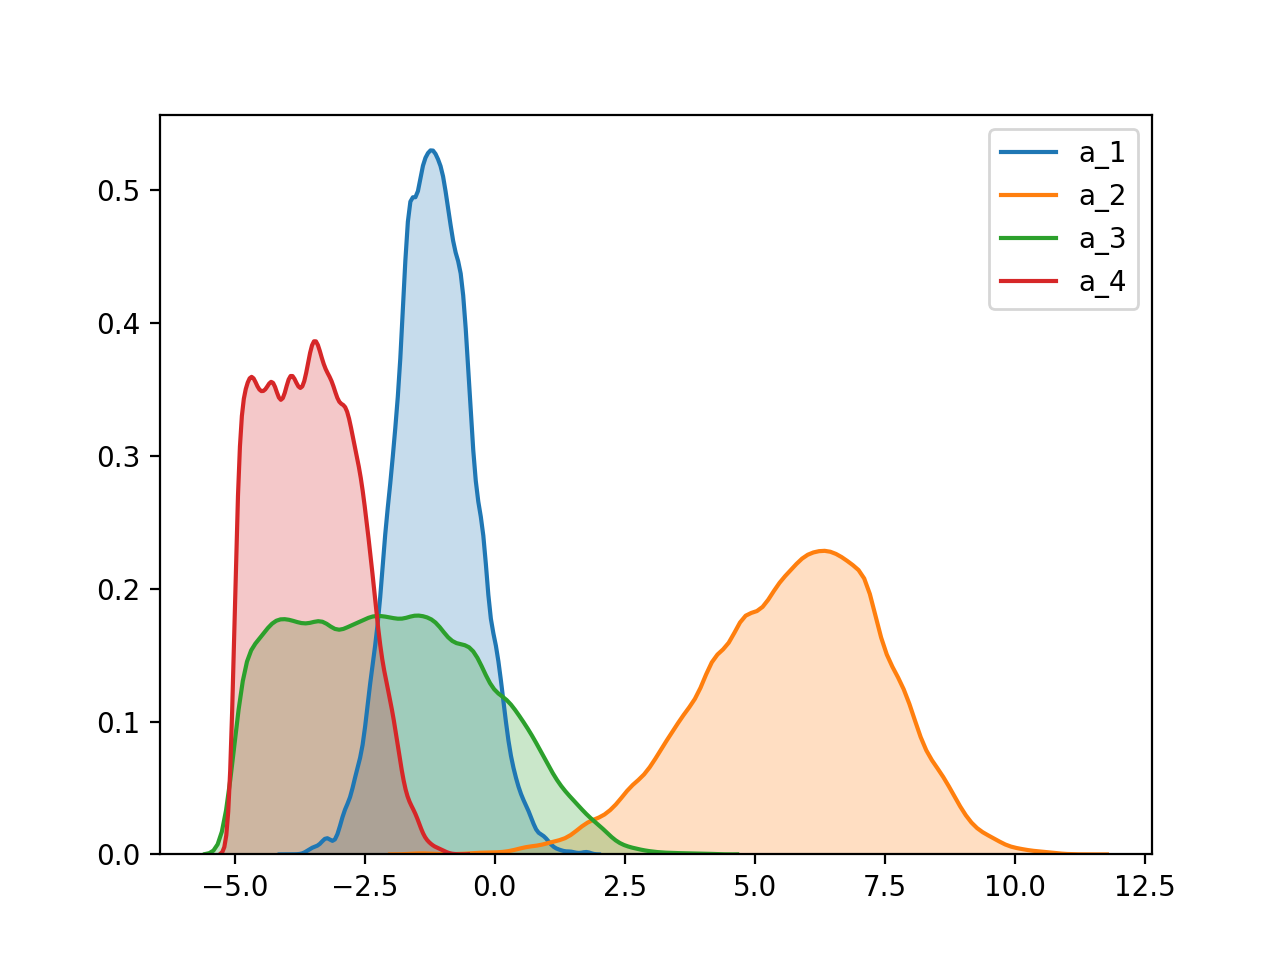
\includegraphics[width=0.5\textwidth]{./figures/poly_posteriors_m0.png} &
    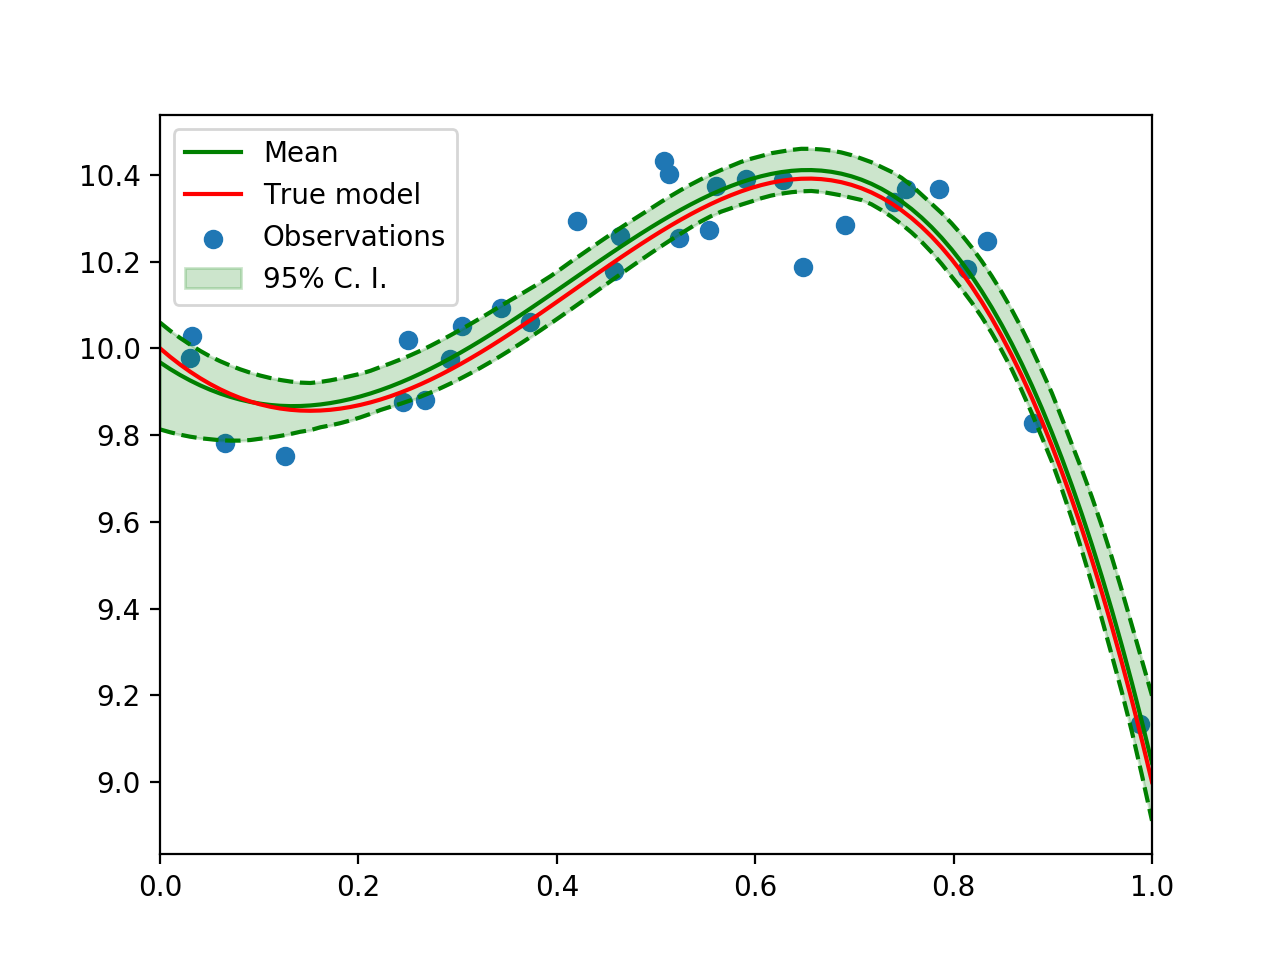
\includegraphics[width=0.5\textwidth]{./figures/poly_predict_check.png}
    \end{tabular}}
    \caption{Left: marginal posterior distributions for parameters $a_{1,...,4}$ for the polynomial model. Right: posterior predictive check.}
    \label{fig:poly}
\end{figure}

\noindent \textbf{\small Forward uncertainty propagation (\texttt{Fprop}).} In this module, we include a simple polynomial chaos construction. The example included is the polynomial chaos expansion of a uniform distribution based on canonical Gaussian distributions $\mathcal{N}(0,1)$. \\

\noindent \textbf{\small Applications (\texttt{Applications}).} We include different examples of applications. First, we introduce a test case with an adiabatic reactor of a simple mixture. Examples on the particular applications of my thesis will be also included here.\\

\noindent \textbf{\small Adiabatic reactor.} In this example, we use the python implementation of the physico-chemical library Mutation++\footnote{\url{https://github.com/mutationpp/Mutationpp}} to compute the time evolution of the temperature for an air5 $\{\mathrm{N, NO, O, O_{2}, N_{2}}\}$ adiabatic reactor. The results in terms of the Sobol indices evolution with time is shown in Fig.~\ref{fig:ad_react_SA}. In the legend, the chemical mechanism considered for such mixture is shown.

\begin{figure}[!htb]
    \centering{
    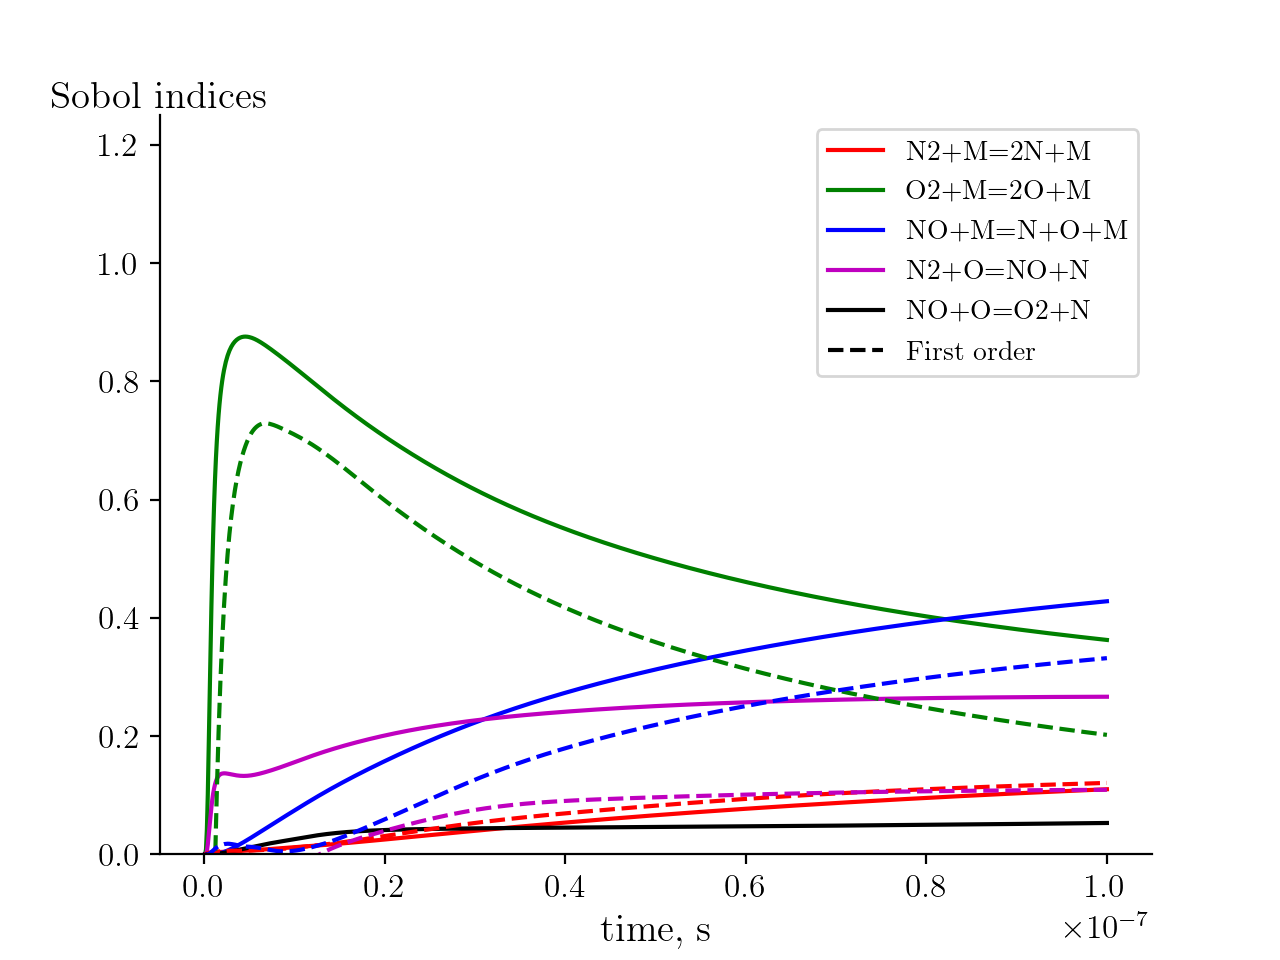
\includegraphics[width=0.7\textwidth]{./figures/Sobol_10000.png}
    \caption{Time evolution of the first order and total order Sobol indices for the variance-based sensitivity of the temperature evolution of an air5 adiabatic reactor at 100 hPa with respect to the pre-exponential factors of the reaction rates of the chemical mechanism.}}
    \label{fig:ad_react_SA}
\end{figure}

For such example, the reaction rates were sampled from log-uniform distributions with the hyperparameters shown in Table~\ref{tab:react_dist}. They have been chosen to encompass their current value according to the chemical model of Park, and also with a variability that does not produce instabilities in the solver in Mutation++. The Sobol indices are based on a Monte Carlo estimate with 10,000 samples. This example is just to demonstrate how SoFIA can be coupled to other libraries to produce various results. The implementation has been sped-up by using parallelization via the module \texttt{mpi4py}.

\begin{table}[!hbt]
    \centering
    \caption{Probability distributions for the pre-exponential factors of the reaction rates of an air5 chemical mechanism.} 
    \label{tab:react_dist}
      \begin{tabular}{l  l}
        \toprule
        Variables  & distribution \\ \midrule
        $\log A_{\mathrm{N_{2}+M \rightleftharpoons 2N+M}}$ & $\mathcal{U}[20,22]$ \\
        $\log A_{\mathrm{O_{2}+M \rightleftharpoons 2O+M}}$ & $\mathcal{U}[20,22]$ \\
        $\log A_{\mathrm{NO+M \rightleftharpoons N+O+M}}$ & $\mathcal{U}[10,15]$ \\
        $\log A_{\mathrm{N_{2}+O \rightleftharpoons NO+N}}$ & $\mathcal{U}[10,15]$ \\
        $\log A_{\mathrm{NO+O \rightleftharpoons O_{2}+N}}$ & $\mathcal{U}[10,15]$
    
      \end{tabular}
\end{table}

A forward propagation of the a priori uncertainty imposed on the reaction rates of the adiabatic reactor was also carried out (Fig.~\ref{fig:ad_react_Fprop}). Notice that the initial temperature was considered certain in all cases. The contributions to the overall uncertainty shown in Fig.~\ref{fig:ad_react_Fprop} are mainly due to the reactions with the highest Sobol indices shown in Fig.~\ref{fig:ad_react_SA}.

\begin{figure}[!htb]
    \centering{
    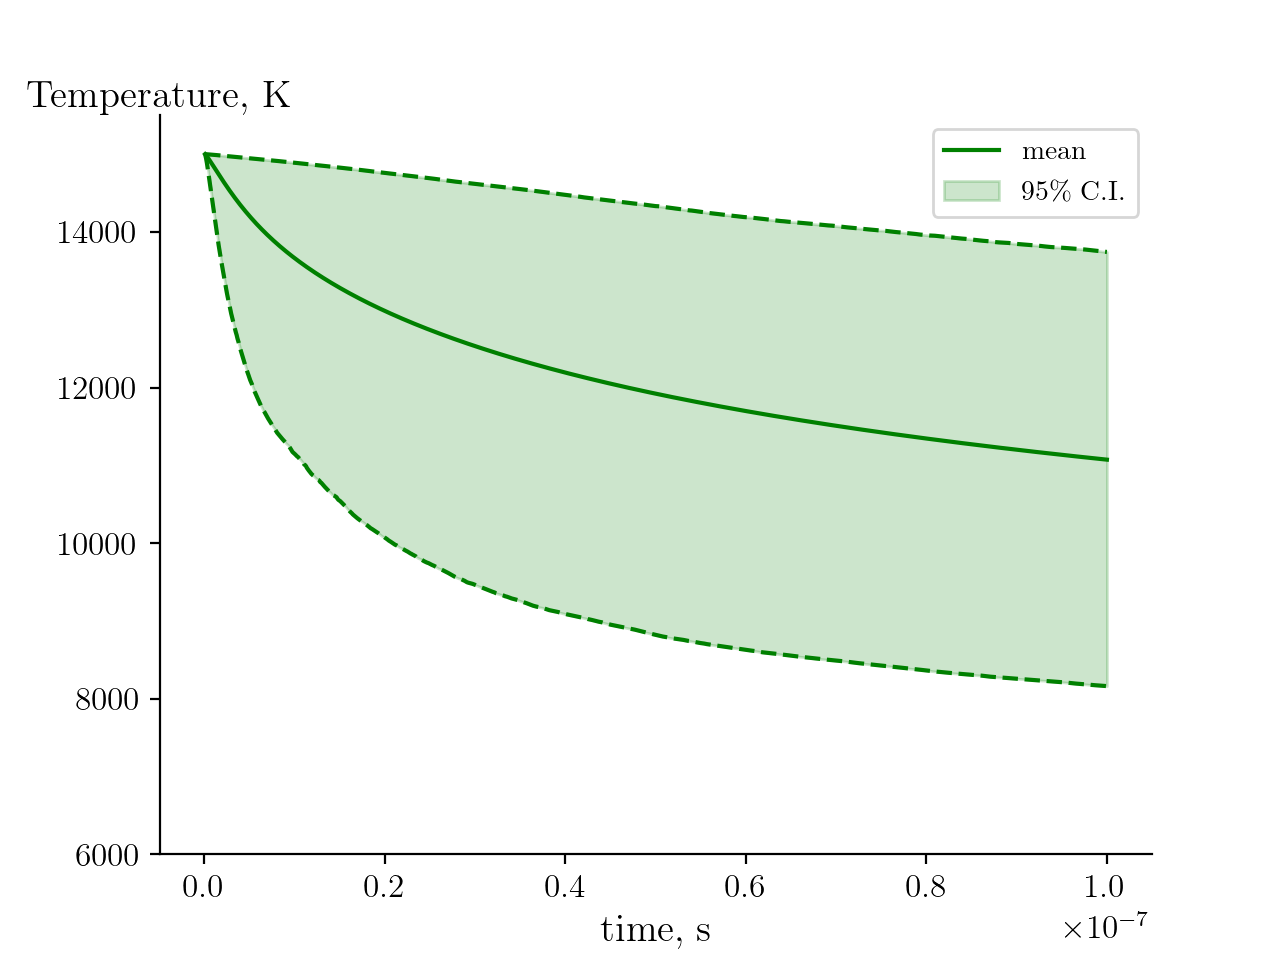
\includegraphics[width=0.7\textwidth]{./figures/temp_adi_reactor_p100.png}
    \caption{Time evolution of the mean and 95\% confidence interval of the temperature of an air5 adiabatic reactor at 100 hPa when reaction rates are considered uncertain following Table~\ref{tab:react_dist} distributions.}}
    \label{fig:ad_react_Fprop}
\end{figure}

If experimental data are available, the uncertainty estimate can be refined and attain objectivity. The following Fig.~\ref{fig:ad_react_Iprop} shows two different cases. The left plot shows the predictive performance of the calibrated model based on one data point, while the plot on the right uses 5 data points randomly distributed in time. The calibration is performed with 10,000 burned samples and a further 10,000 chain samples. The noise of the observation is $\sigma = 100 \ K$.

\begin{figure}[!htb]
    \centerline{
    \begin{tabular}{c c}
    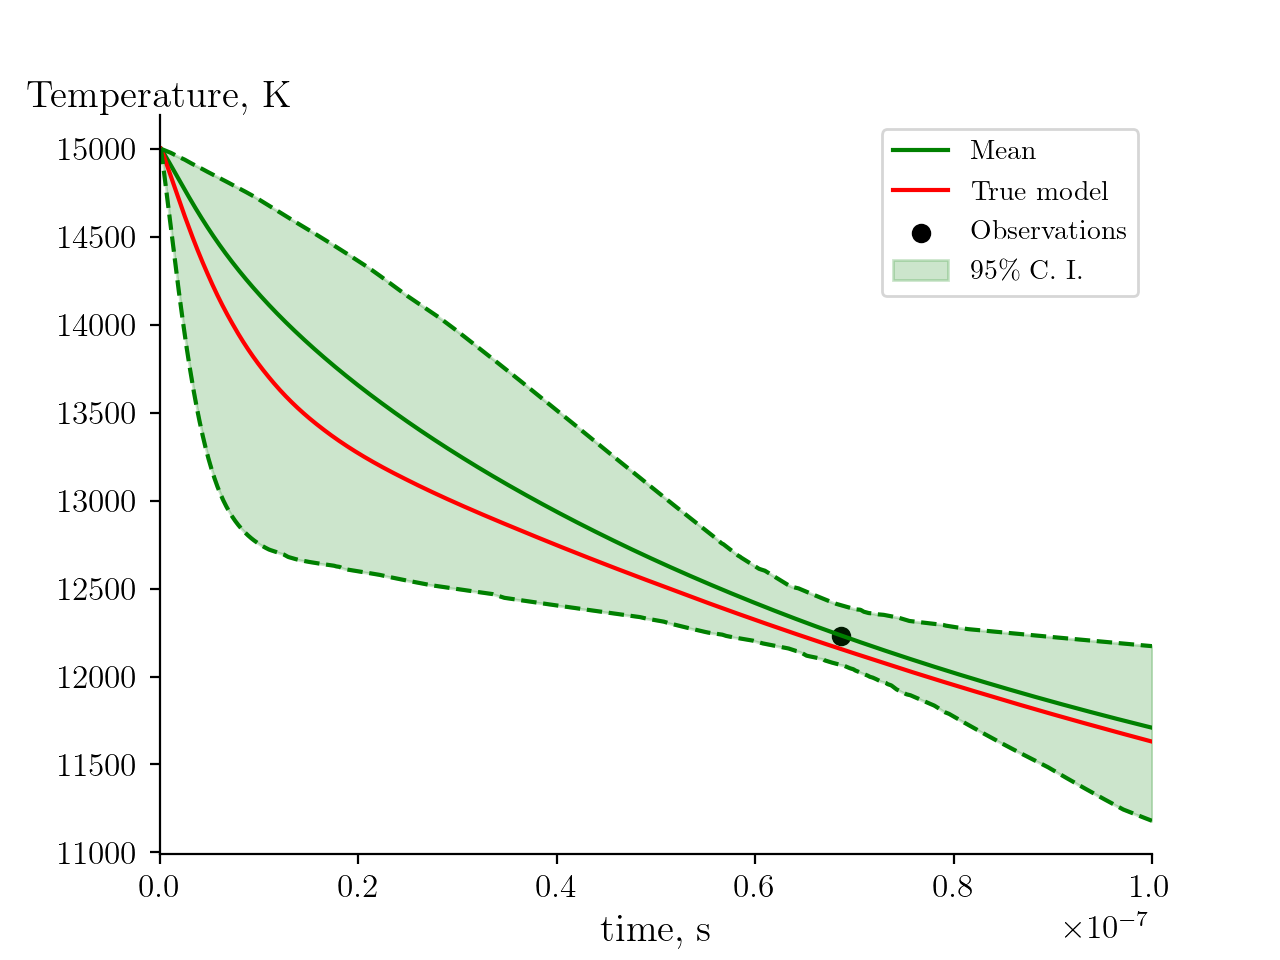
\includegraphics[width=0.5\textwidth]{./figures/Iprop_ad_react_1obs.png} &
    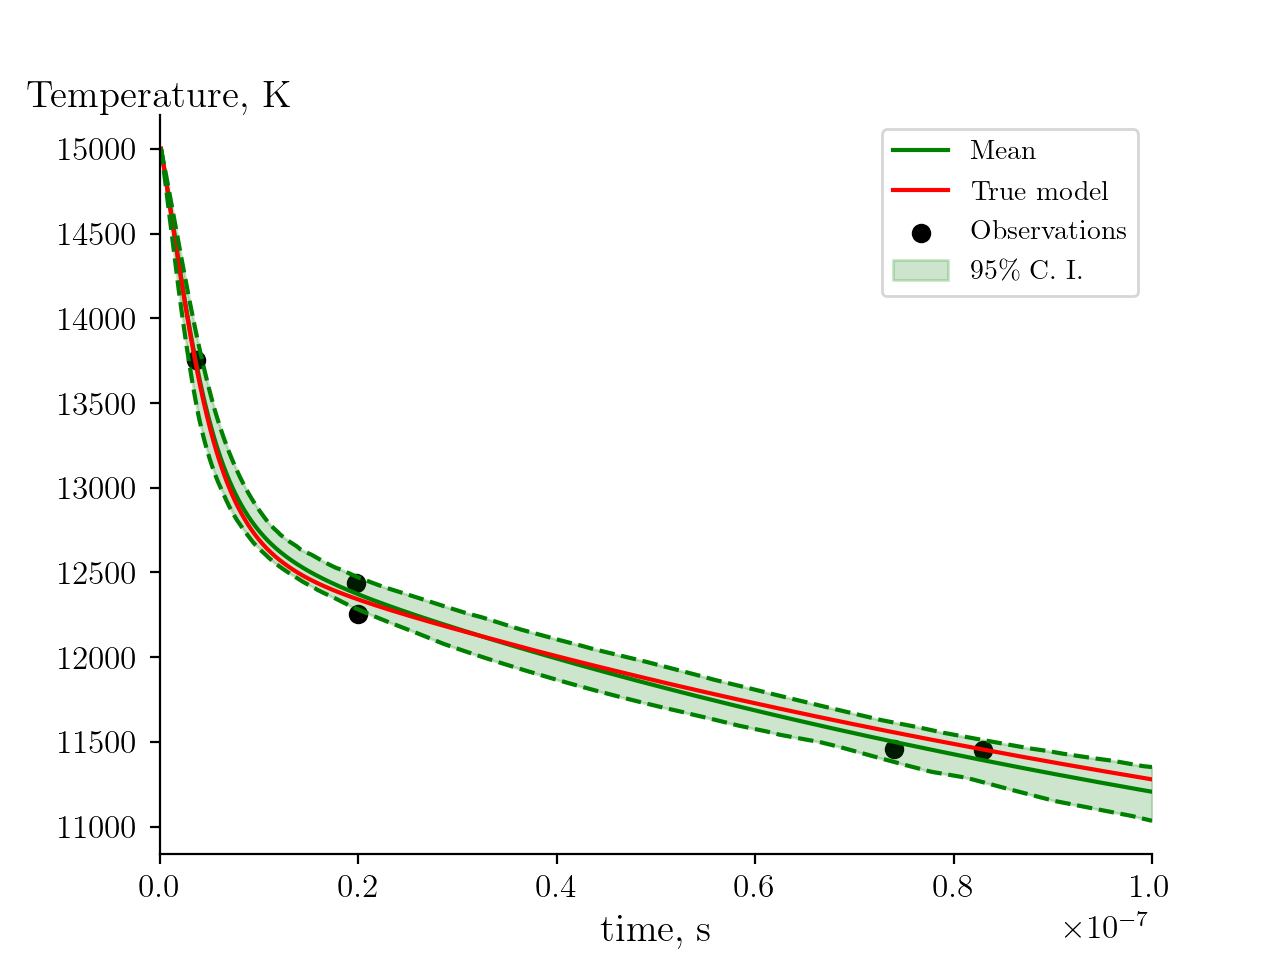
\includegraphics[width=0.5\textwidth]{./figures/Iprop_ad_react_10000.png}
    \end{tabular}}
    \caption{Left: posterior predictive check of the calibrated model with 1 observation. Right: posterior predictive check of the calibrated model with 5 observations.}
    \label{fig:ad_react_Iprop}
\end{figure}

Further, we also include the computed marginal posterior distributions of the pre-exponential factors in Fig.~\ref{fig:ad_react_Iprop_marginals}. Notice that for the case with 5 observations, the best learned parameter is the one attached to the reaction with the largest the Sobol indices, which dominates the temperature estimation in all the time span. The other coefficients can be known to a lesser degree, some still covering the whole prior range. The plots are given in logarithmic range.\\

\begin{figure}[!htb]
    \centerline{
    \begin{tabular}{c c}
    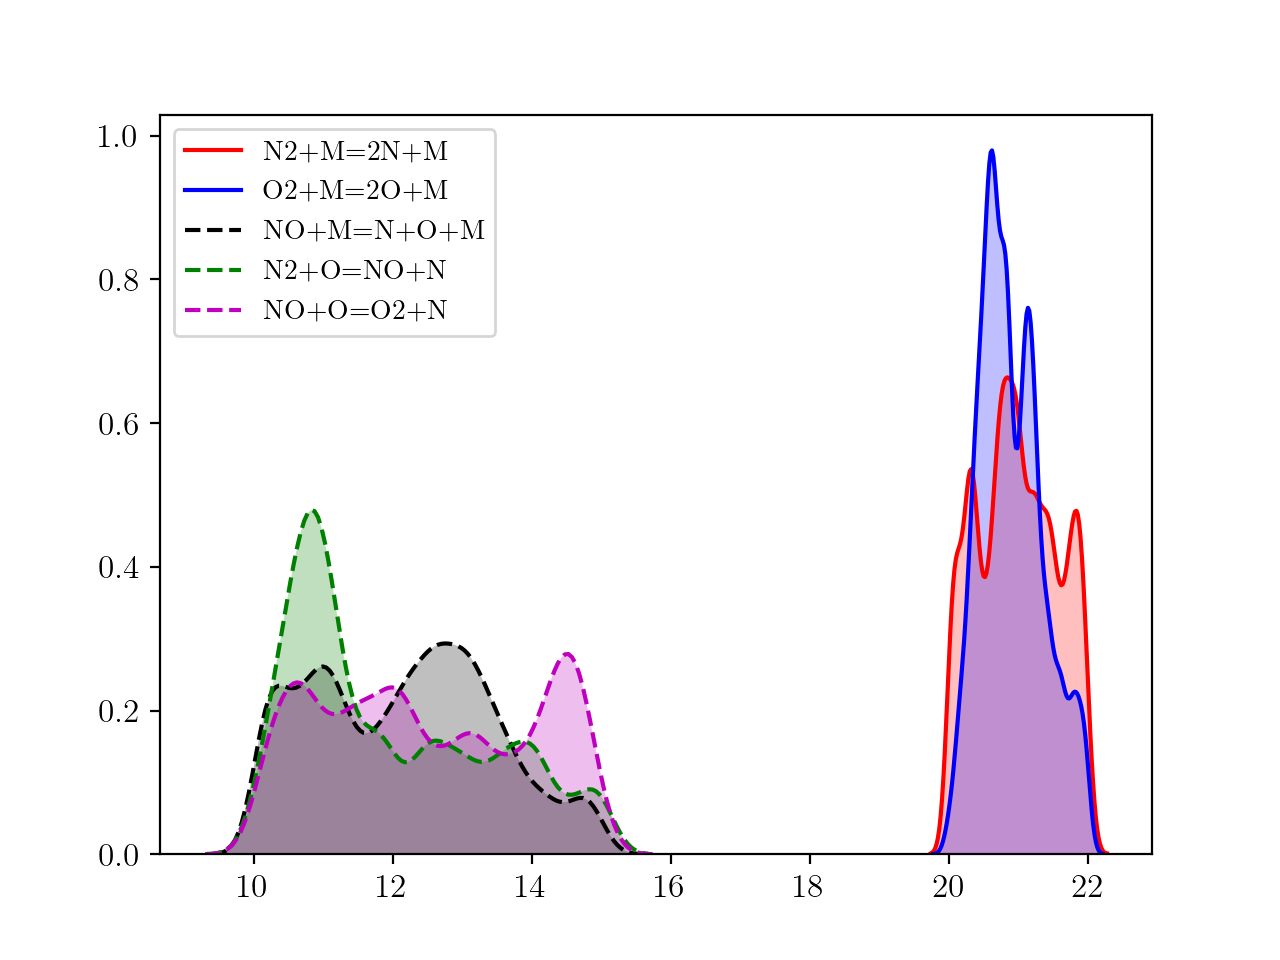
\includegraphics[width=0.5\textwidth]{./figures/marginals_1obs.png} &
    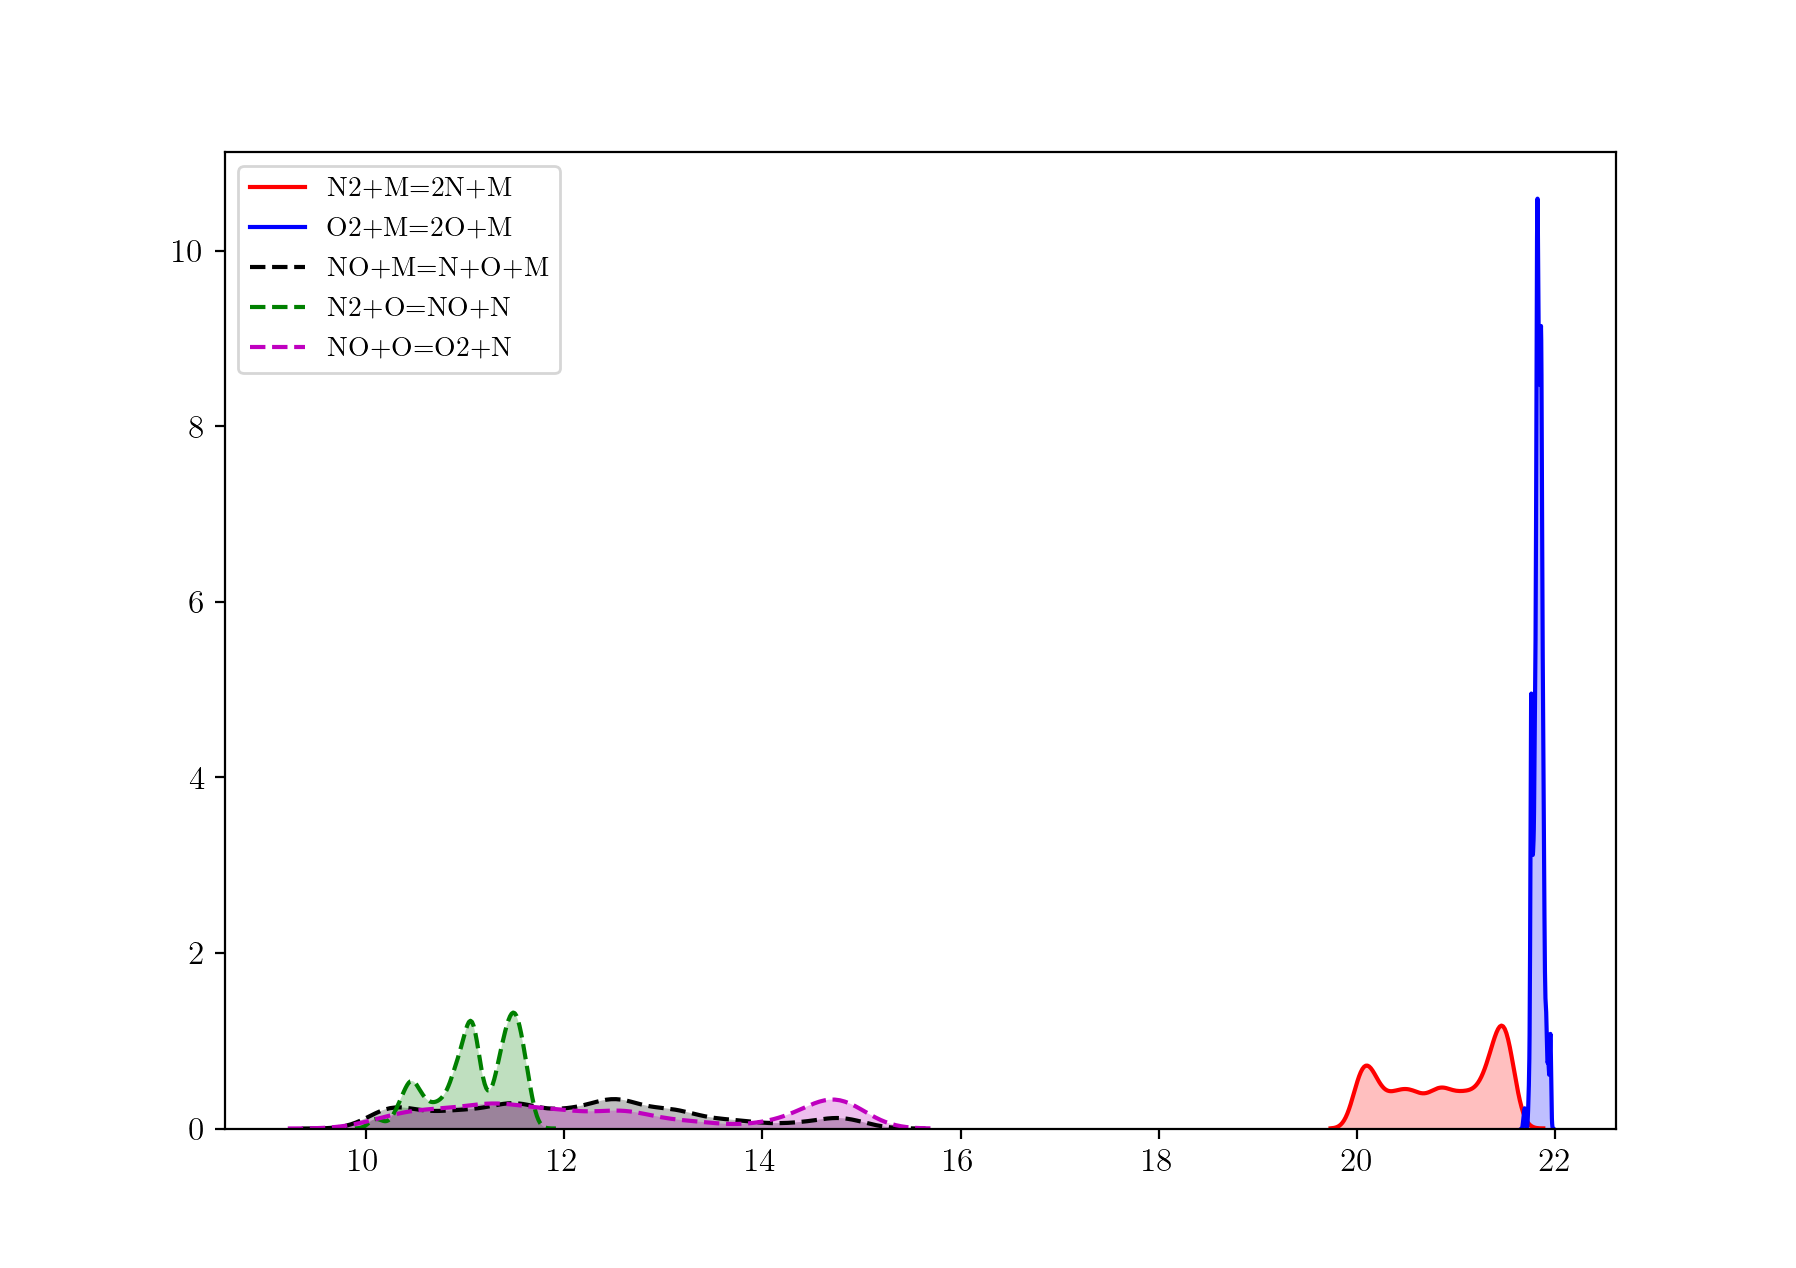
\includegraphics[width=0.53\textwidth]{./figures/posteriors.png}
    \end{tabular}}
    \caption{Left: resulting marginal posterior distributions of the calibrated pre-exponential factors with 1 observation. Right: resulting marginal posterior distributions of the calibrated pre-exponential factors with 5 observations.}
    \label{fig:ad_react_Iprop_marginals}
\end{figure}

It is also interesting to see that for an adiabatic reactor with a perfectly known initial temperature and a measurement of the temperature at steady-state, NO dissociation is quite well defined, given that it governs the temperature evolution at later times, unlike oxygen dissociation. Fig.~\ref{fig:ad_react_Iprop_marginals_steady} shows the posterior predictive and the resulting marginal distributions.

\begin{figure}[!htb]
    \centerline{
    \begin{tabular}{c c}
    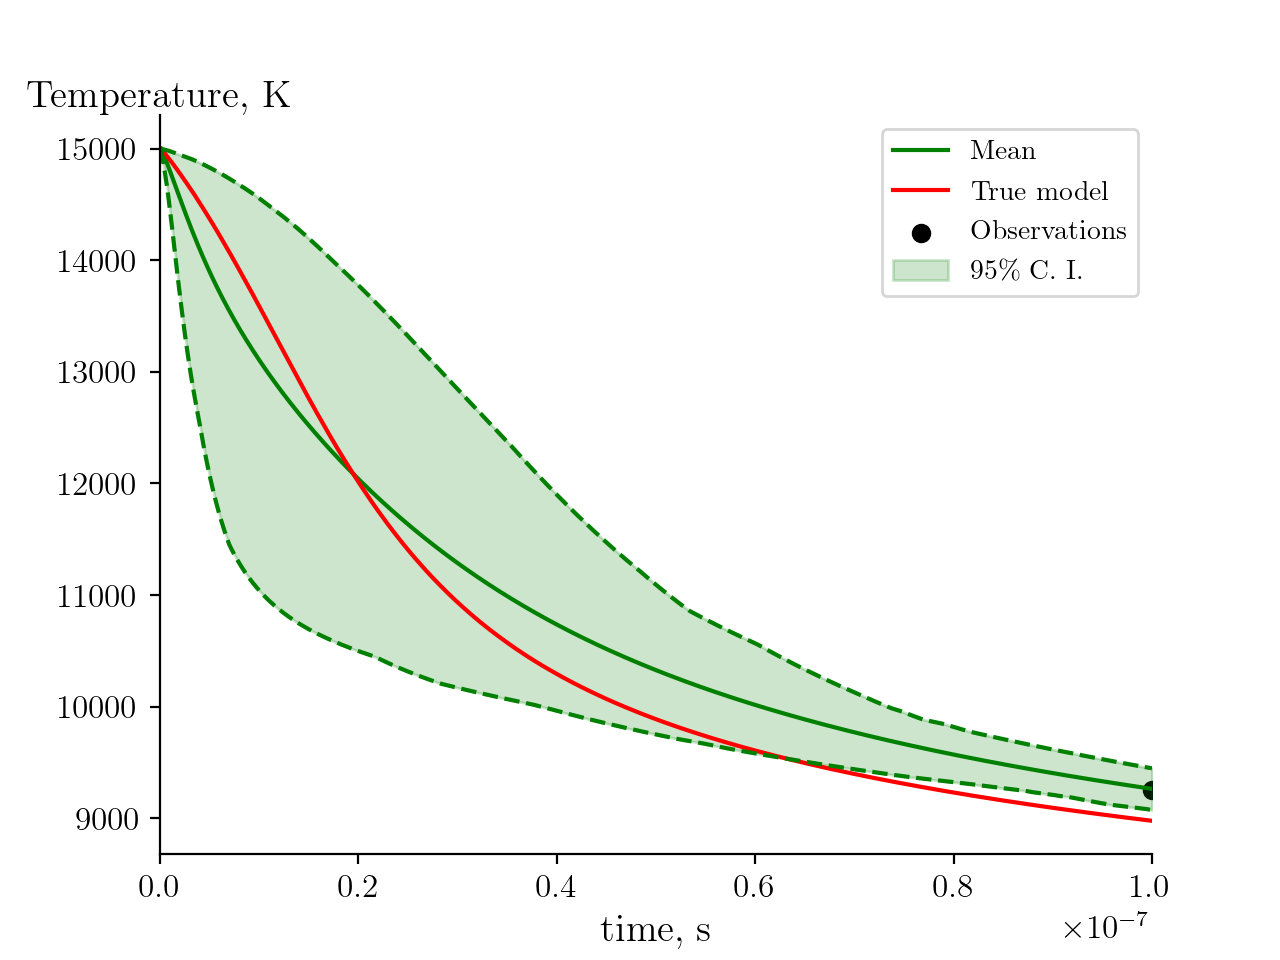
\includegraphics[width=0.5\textwidth]{./figures/Iprop_steady_point.png} &
    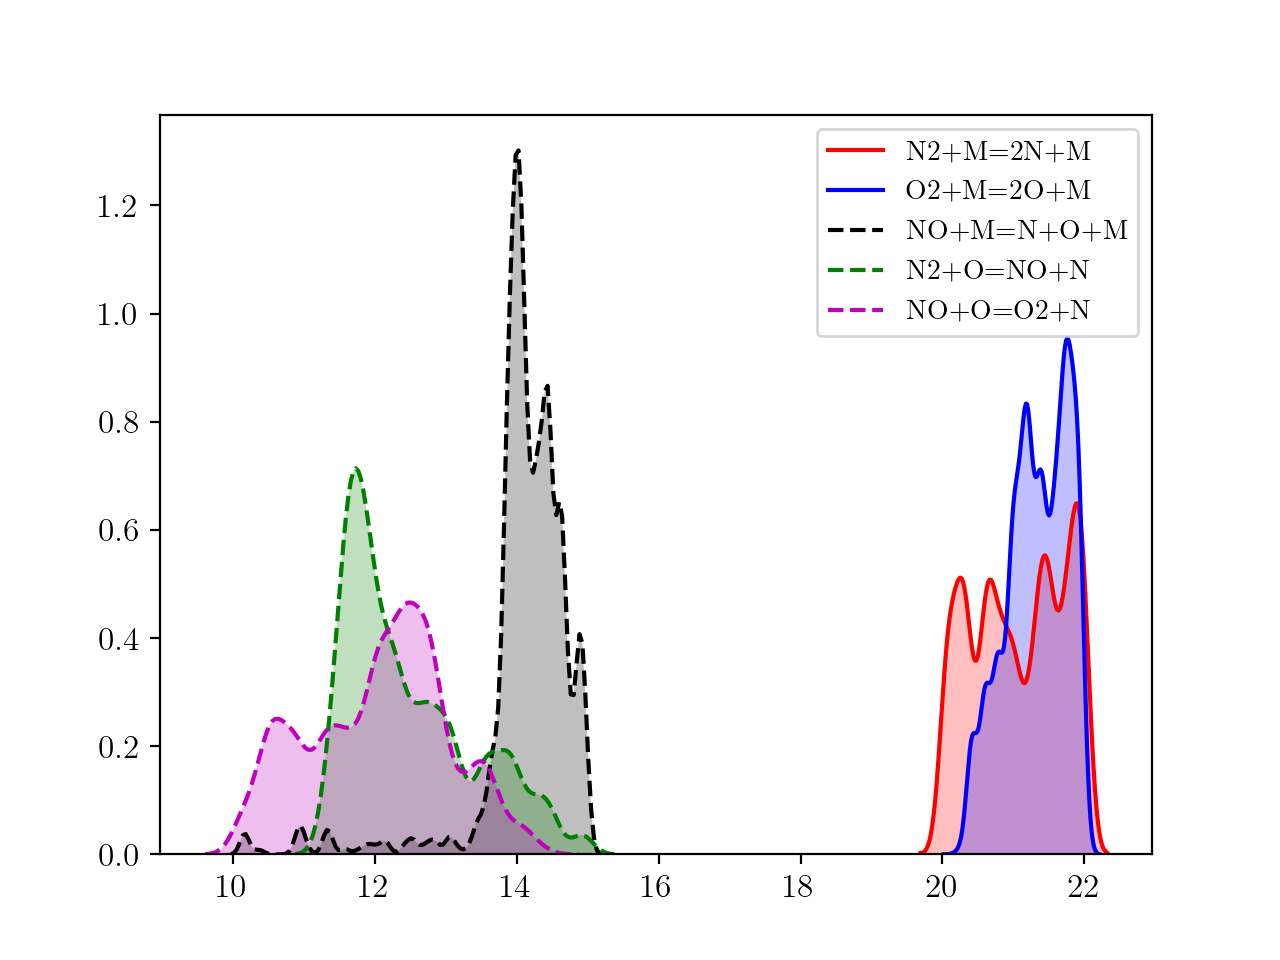
\includegraphics[width=0.53\textwidth]{./figures/marginals_steady_point.png}
    \end{tabular}}
    \caption{Left: posterior predictive check of the calibrated model with 1 observation at steady-state. Right: resulting marginal posterior distributions of the calibrated pre-exponential factors.}
    \label{fig:ad_react_Iprop_marginals_steady}
\end{figure}

All of the above results assume perfect knowledge of the initial temperature. If we know consider the initial temperature to be unknown within some wide bounds $T_{\mathrm{init}} \sim \mathcal{U}[10000,15000]$, the latest results of Fig.~\ref{fig:ad_react_Iprop_marginals_steady} would now be the ones in Fig.~\ref{fig:ad_react_Iprop_marginals_steady_Tinit}. Notice the change in the calibrated model as well as the marginal distributions. 

\begin{figure}[!htb]
    \centerline{
    \begin{tabular}{c c}
    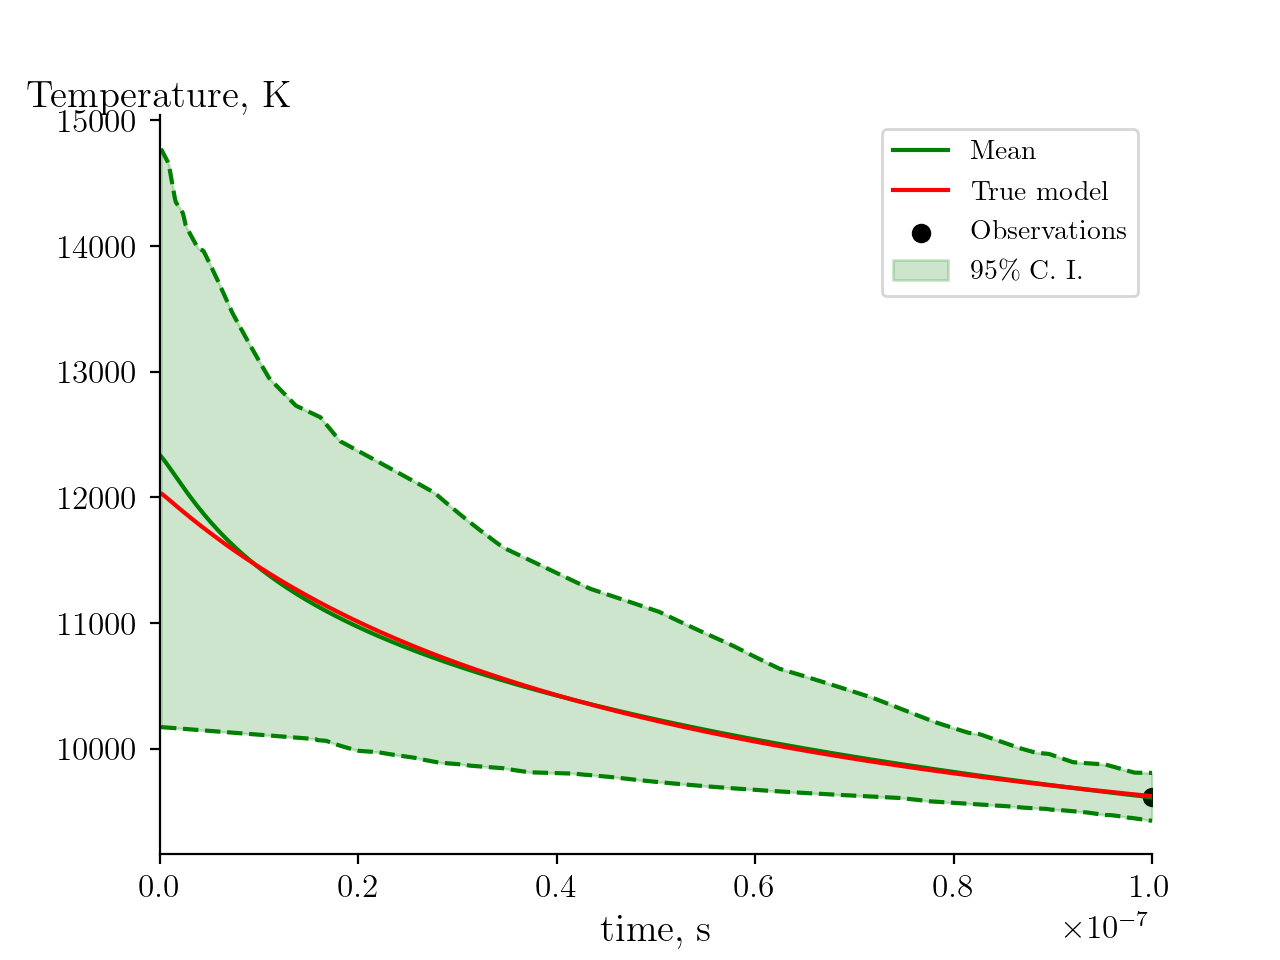
\includegraphics[width=0.5\textwidth]{./figures/Iprop_post_check_10000_steady_Tinit.png} &
    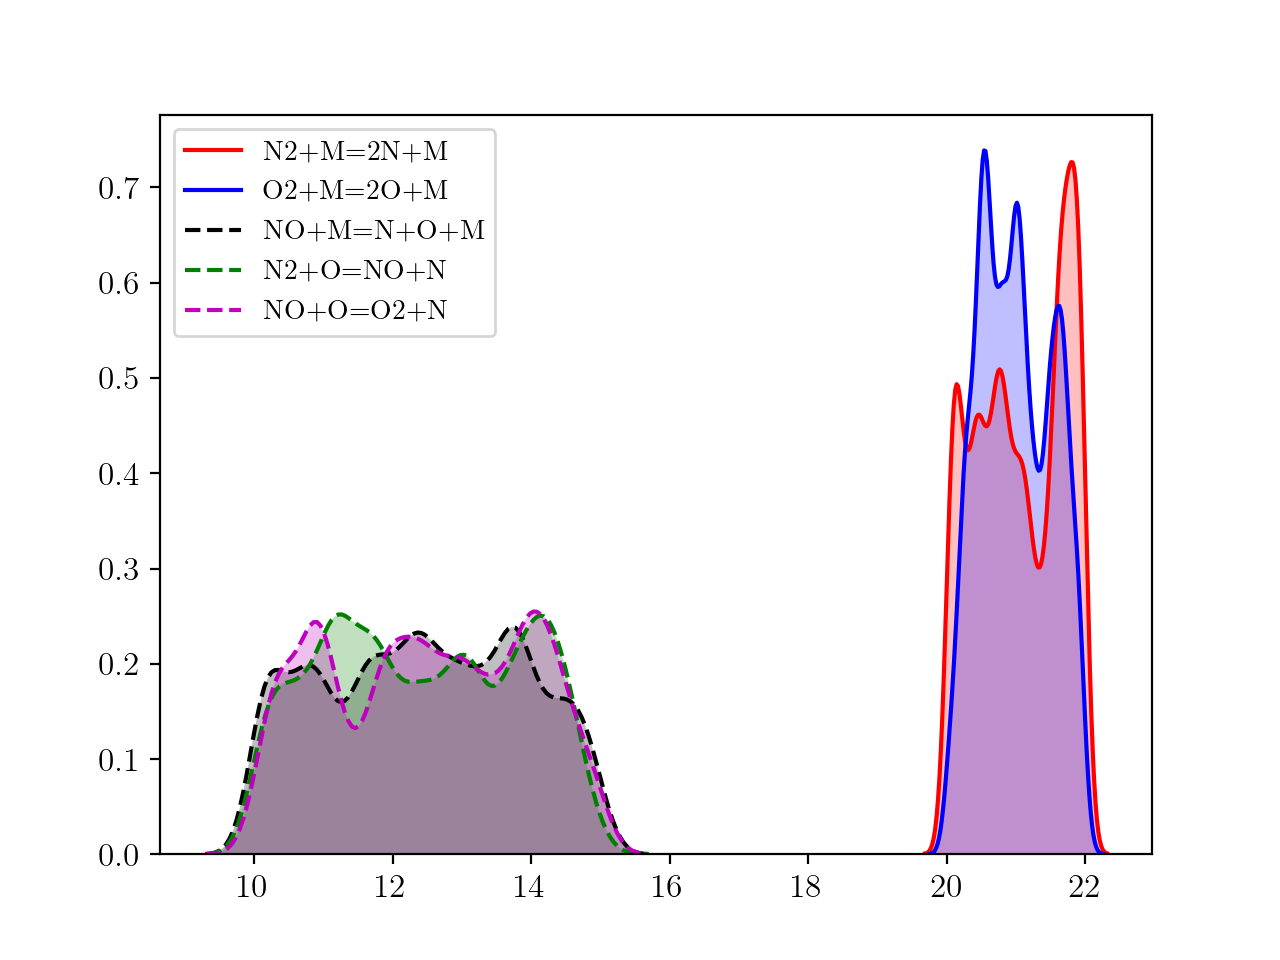
\includegraphics[width=0.53\textwidth]{./figures/marginals_10000_Tinit.png}
    \end{tabular}}
    \caption{Left: posterior predictive check of the calibrated model with 1 observation at steady-state. Right: resulting marginal posterior distributions of the calibrated pre-exponential factors.}
    \label{fig:ad_react_Iprop_marginals_steady_Tinit}
\end{figure}

If we were to run a sensitivity analysis again, this time with the initial temperature as a free parameter, we would see the following result of Fig.~\ref{fig:ad_react_SA_Tinit2}. In it, we can appreciate how the sensitivity indices change values once the initial temperature is considered unknown. The marginal posterior distributions changes can be understood based on the sensitivity of the problem when adding the initial temperature as an additional free parameter.\\

\begin{figure}[!htb]
    \centering{
    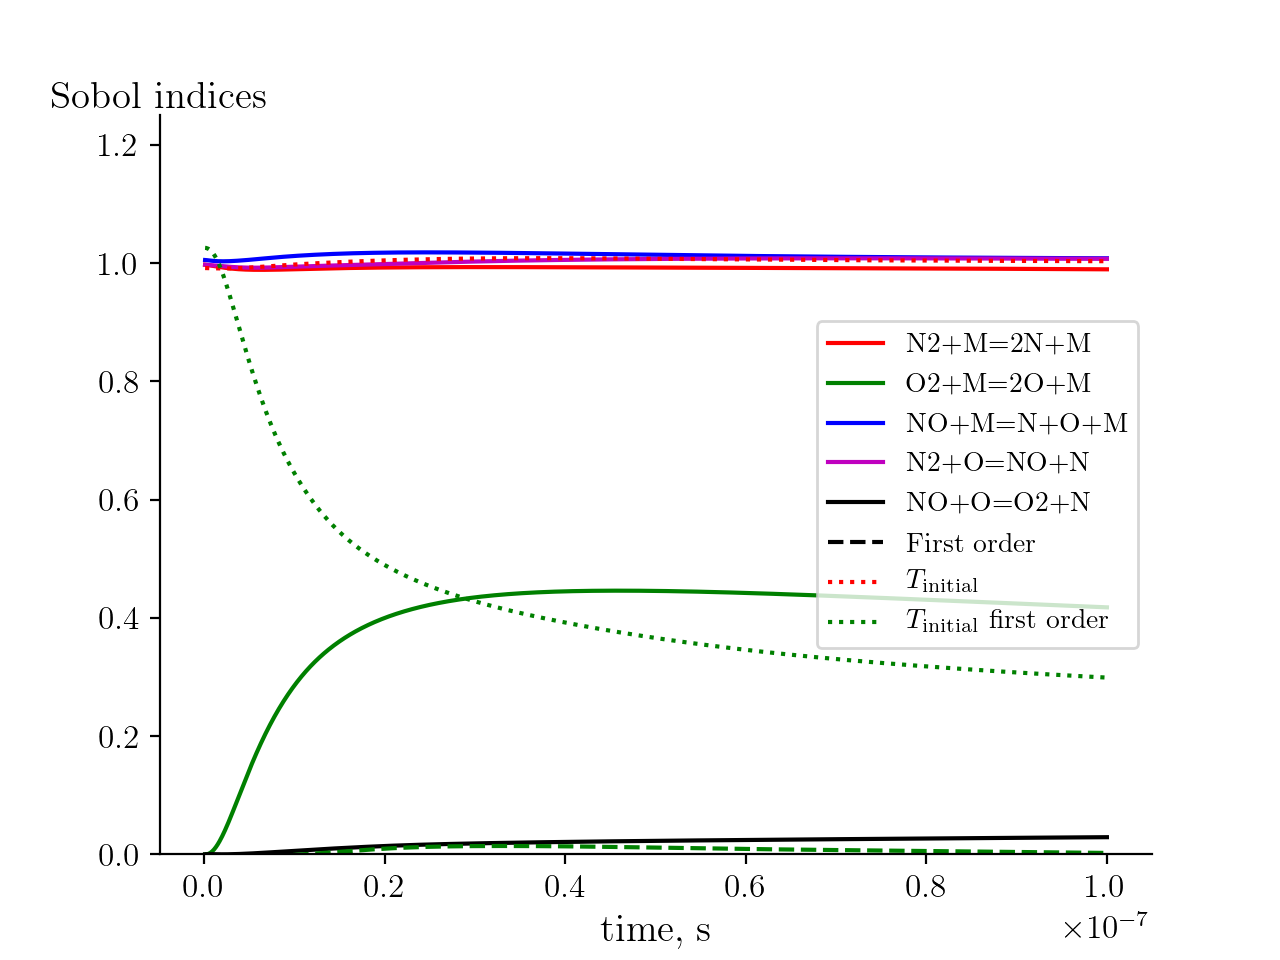
\includegraphics[width=0.7\textwidth]{./figures/Sobol_Tinit.png}
    \caption{Time evolution of the first order and total order Sobol indices for the variance-based sensitivity of the temperature evolution of an air5 adiabatic reactor at 100 hPa with respect to the pre-exponential factors of the reaction rates of the chemical mechanism and the initial temperature.}}
    \label{fig:ad_react_SA_Tinit2}
\end{figure}

\noindent \textbf{Heterogeneous catalysis for reusable TPS ground testing and enthalpy rebuilding.} This application pertains to my PhD thesis work. We calibrate a chemically reacting flow model in chemical non-equilibrium with plasma wind tunnel experimental data. We look for the resulting uncertainty on the catalytic coefficients of the different materials tested for each independent experimental run as well as the free stream boundary condition (enthalpy). For more technical details see footnote\footnote{A. del Val, Bayesian calibration and assessment of gas-surface interaction models and experiments in atmospheric entry plasmas, IPP/VKI, 2021 - \url{www.doi.org/10.13140/RG.2.2.27055.82089}}.

In SoFIA, in the \texttt{Applications/catalysis/models} folder, we include the saved Gaussian Process (GP) models for each experimental run of names \texttt{MTAt1,2,...}. These GP models are built to approximate the log-likelihood functions of the experiments. In turn, such models are used to run an MCMC algorithm and compute the marginal posterior distributions of the quantities of interest (catalytic efficiency parameters). Such posterior distributions are propagated through another set of GP surrogates with the names \texttt{H\_case\_name.sav} to obtain the rebuilt free stream enthalpy.

Two major ``ingredients'' are used for the computation of the posterior in \texttt{computation\_posterior.py} the \texttt{json} file \texttt{models.json}, and the file \texttt{data\_assembly\_cat.py}. \\

\noindent The file \texttt{models.json} contains a dictionary where the models can be called together with the priors used for their input variables and the order of the inputs to the model in the form of indexes (\texttt{inputs} in the \texttt{json} file dictionary).\\

\noindent The file \texttt{data\_assembly\_cat.py} contains the class to assemble the likelihood function needed for the subsequent Bayesian analysis. In it, the log-likelihood function is loaded the hyperparameters for the different priors as well as de-normalization of the inputs are specified.\\

\noindent To run completely new cases, the \textbf{suggested workflow} is as follows:

\begin{enumerate}
    \item Run the optimal algorithm in a grid of points \\
    (\texttt{catalysis/}\texttt{utilities/}\texttt{sampler}\texttt{\_opt}\texttt{\_loglik.py}). This first step is suposed to be custom-made as it will depend on the solver and how it inputs and outputs data. For the particular case of the Boundary Layer Code at VKI, a model script I made is included. This script contains the \texttt{BL} function which computes the heat flux given a set of parameters \texttt{x0} and the catalytic parameters \texttt{gamma} which are vectors. The function \texttt{functional} is the function to minimize, it is the negative log-likelihood function. The important snippet of this script is the \texttt{main loop} which basically goes over the grid of gamma values and finds the optimal values of the log-likelihood function by searching on \texttt{x0}. The values of \texttt{x0} and \texttt{gamma}, together with the negative log-likelihood values are written in the file \texttt{output.out}. NOTE: We are looking for the maximizers of the log-likelihood function. As we use an optimization algorithm (Nelder-Mead) which minimizes an objective function, we change the sign of the log-likelihood function to be the negative log-likelihood function, and this is the value that is printed out in \texttt{output.out}.
    \item Use \texttt{catalysis/models/save\_GP.py} and \texttt{catalysis/models/save\_H\_GP.py} to save GP models that approximate the optimal log-likelihood function and the optimal enthalpy based on the points previously computed. NOTE: You can do this either with the implemented \texttt{SoFIA/utilities/GPR} module or with the \textit{scikit-learn} library.
    \item In the file \texttt{catalysis/models/models.json}, save the data of your case.
    \item Use the model to compute the posterior distribution and obtain the resulting chain from the MCMC algorithm with \texttt{catalysis/computation\_posterior.py}. The resulting MCMC chain can be used in \texttt{catalysis/computation\_H\_optimal.py} to compute the $H^{\mathrm{opt}}$ enthalpy.
    \item Check diagnostics.
    \item Re-run additional points of the optimal log-likelihood algorithm in the area where MCMC drew points in a Monte Carlo fashion.
    \item Start from point 2.
\end{enumerate}

\textbf{Proposed diagnostics.} A tricky issue may arise for non-experts in these analyses. The workflow described cannot be run blindly, without thoroughly assessing the quality of the results. As this requires some in-depth knowledge of the analyses, I propose here a quick way of checking if the GP surrogate + MCMC sampling give reasonable results or if the surrogate estimation would need additional points. There are two sources of problems in this procedure. Once we have a GP surrogate of the optimal log-likelihood to work with, we need to check if the MCMC chain is converged. For this, 3 different diagnostics are presented in \texttt{Docs/jup\_notebooks/catalysis\_demo.py}. We compute the acceptance rate, we plot the trace of the chain and the autocorrelation function. That is enough to have a thorough assessment. Second, the GP surrogate might not be good at all, for this purpose we propose the following: plot the chain samples on the S-curves as done at the end of the script in \texttt{Docs/jup\_notebooks/catalysis\_demo.py}. This gives you a quick view of the samples drawn from the posterior and you can check whether or not they are in an area where they would be expected to be. If you know the chain is converged but the samples just don't really follow the S-curves or seem to be in weird places, this is most likely due to a bad surrogate. In such case, go back to the code and add a few extra points until this last diagnostics is satisfactory.\\

\noindent \textbf{Nitrogen ablation.} This is another application that falls from my PhD work. We calibrate a chemically reacting flow model in chemical non-equilibrium with plasma wind tunnel experimental data. We look for the resulting uncertainty on the nitridation reaction efficiencies for each independent experimental run. We do this with different models that encapsulate different assumptions. For more technical details see footnote\footnote{A. del Val, Bayesian calibration and assessment of gas-surface interaction models and experiments in atmospheric entry plasmas, IPP/VKI, 2021 - \url{www.doi.org/10.13140/RG.2.2.27055.82089}}.

In SoFIA, in the \texttt{Applications/nitridation/models} folder, we include the saved Gaussian Process (GP) models for each experimental run of names \texttt{G4,5,...}. These GP models are built to approximate the logarithm of the recession rate and CN densities measured in the boundary layer. In turn, such models are used to run an MCMC algorithm and compute the marginal posterior distributions of the quantities of interest (nitridation efficiency parameters). The file \texttt{nitridation/models/models.json} contains dictionaries that basically index the location of the models to be loaded for each physical model and experimental case of interest. Further, the file \texttt{nitridation/cases.json} contains the experrimental data and Non-Dimensional Parameters (NDPs) for each case.

For an example on how to run nitridation cases, refer to \texttt{SoFIA/Docs/jup\_notebooks/env/nitridation\_demo.ipynb}.

To run completely new cases the \textbf{suggested workflow} is as follows:

\begin{enumerate}
    \item Run the model in a grid of points
\end{enumerate}


\end{document}